% Created 2026-04-21 Tue 19:37
% Intended LaTeX compiler: lualatex
\DocumentMetadata{lang = en, pdfversion = 2.0, pdfstandard = ua-2, pdfstandard = a-4, testphase = {phase-III, title, table, math, firstaid}}
\documentclass[11pt]{article}
\usepackage{amsmath}
\usepackage{fontspec}
\usepackage{graphicx}
\usepackage{longtable}
\usepackage{wrapfig}
\usepackage{rotating}
\usepackage[normalem]{ulem}
\usepackage{capt-of}
\usepackage{hyperref}
\usepackage[margin=1in]{geometry}
\usepackage{fontspec}
\usepackage{verbatim, multicol, tabularx,}
\usepackage{amsmath, amsthm, amssymb, stmaryrd, latexsym, bm, listings, qtree}
\usepackage{framed}
\usepackage{xcolor,colortbl}
\usepackage{media9}
\usepackage[export]{adjustbox}
\usepackage{algorithm}
\usepackage[noend]{algpseudocode}
\usepackage{tikz,pgfplots}
\usetikzlibrary{shapes.geometric}
\let\oldquote=\quote
\let\endoldquote=\endquote
\colorlet{shadecolor}{cyan!15}
\renewenvironment{quote}{\begin{shaded*}\begin{oldquote}}{\end{oldquote}\end{shaded*}}
% From https://tex.stackexchange.com/questions/7032/good-way-to-make-textcircled-numbers
\newcommand*\circled[1]{\tikz[baseline=(char.base)]{\node[shape=circle,draw,inner sep=2pt] (char) {#1};}}
\DeclareMathOperator*{\argmin}{arg\!min}
\DeclareMathOperator*{\argmax}{arg\!max}
\lstset{frame=tb, aboveskip=1mm, belowskip=0mm, showstringspaces=false, columns=flexible, basicstyle={\scriptsize\ttfamily}, numbers=left, frame=single, breaklines=true, breakatwhitespace=true}
\hypersetup{colorlinks=true,urlcolor=blue}
\usepackage{polyglossia}
\setdefaultlanguage[variant=US]{english}
\author{Christopher Simpkins}
\date{Kennesaw State University}
\title{Artificial Intelligence\\\medskip
\large Bayesian Networks}
\hypersetup{
 pdfauthor={Christopher Simpkins},
 pdftitle={Artificial Intelligence},
 pdfkeywords={},
 pdfsubject={Artificial Intelligence Bayesian Networks},
 pdfcreator={Emacs 30.2 (Org mode 9.7.11)}, 
 pdflang={English}}
\begin{document}

\maketitle
\section{Representation of Uncertain Knowledge (AIMA 13.1--13.2)}
\label{sec:org5fee2cb}

A Bayesian network is a directed graph in which each node is annotated with quantitative probability information. The full specification is as follows:

\begin{enumerate}
\item Each node corresponds to a random variable, which may be discrete or continuous.

\item Directed links or arrows connect pairs of nodes. If there is an arrow from node \(X\) to node \(Y\), then \(X\) is said to be a parent of \(Y\). The graph has no directed cycles and hence is a directed acyclic graph, or DAG.

\item Each node \(X_i\) has associated probability information \(\theta(X_i | Parents(X_i))\) that quantifies the effect of the parents on the node using a finite number of parameters.
\end{enumerate}
\section{Bayesian Network Topology}
\label{sec:org1950418}


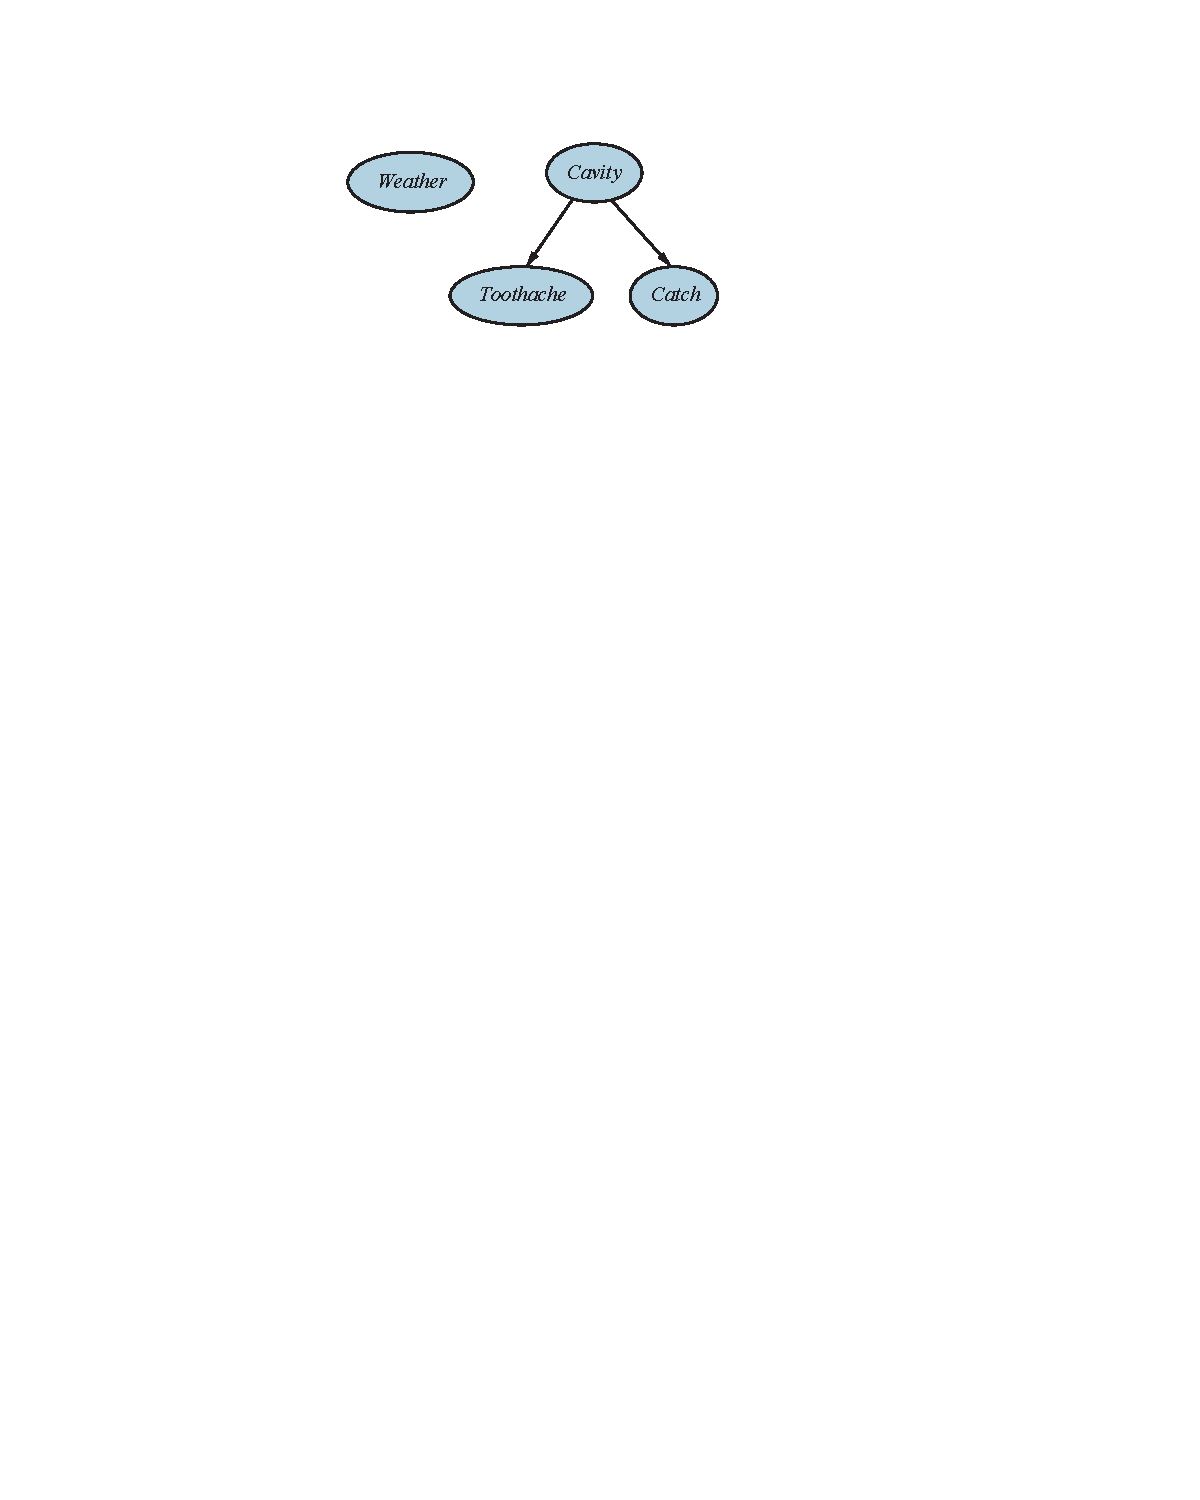
\includegraphics[alt={aima fig 13_01 bayes net weather cavity},width=0.75\linewidth]{aima-fig-13_01-bayes-net-weather-cavity.pdf}


\begin{itemize}
\item The topology of the network -- the set of nodes and links -- specifies the conditional independence relationships that hold in the domain.

\begin{itemize}
\item \(Toothache\) and \(Catch\) are conditionally independent given \(Cavity\).
\end{itemize}

\item Intuitiveley, and arrow \(X \rightarrow Y\) means \(X\) has a direct influence on \(Y\) -- so parents should be \textbf{causes} of effects.
\end{itemize}

It is usually easy for a domain expert to decide what direct influences exist in the domain -- much easier, in fact, than actually specifying the probabilities themselves.
\section{Example: Earthquake vs. Burglary}
\label{sec:org6e3ad7b}

You have a burglar alarm fairly reliable at detecting a burglary, but is occasionally set off by minor earthquakes.

\begin{itemize}
\item Two neighbors, John and Mary, who promise to call when they hear the alarm.
\item John nearly always calls when he hears the alarm, but sometimes confuses the telephone ringing with the alarm and calls then, too.
\item Mary, on the other hand, likes rather loud music and often misses the alarm altogether.
\end{itemize}

Given the evidence of who has or has not called, we would like to estimate the probability of a burglary.
\section{Bayes Net for Earthquake vs. Burglary Reasoning}
\label{sec:orgd851da0}

The \textbf{syntax} of a Bayes net consists of a directed acyclic graph (DAG) with some local probability information attached to each node.


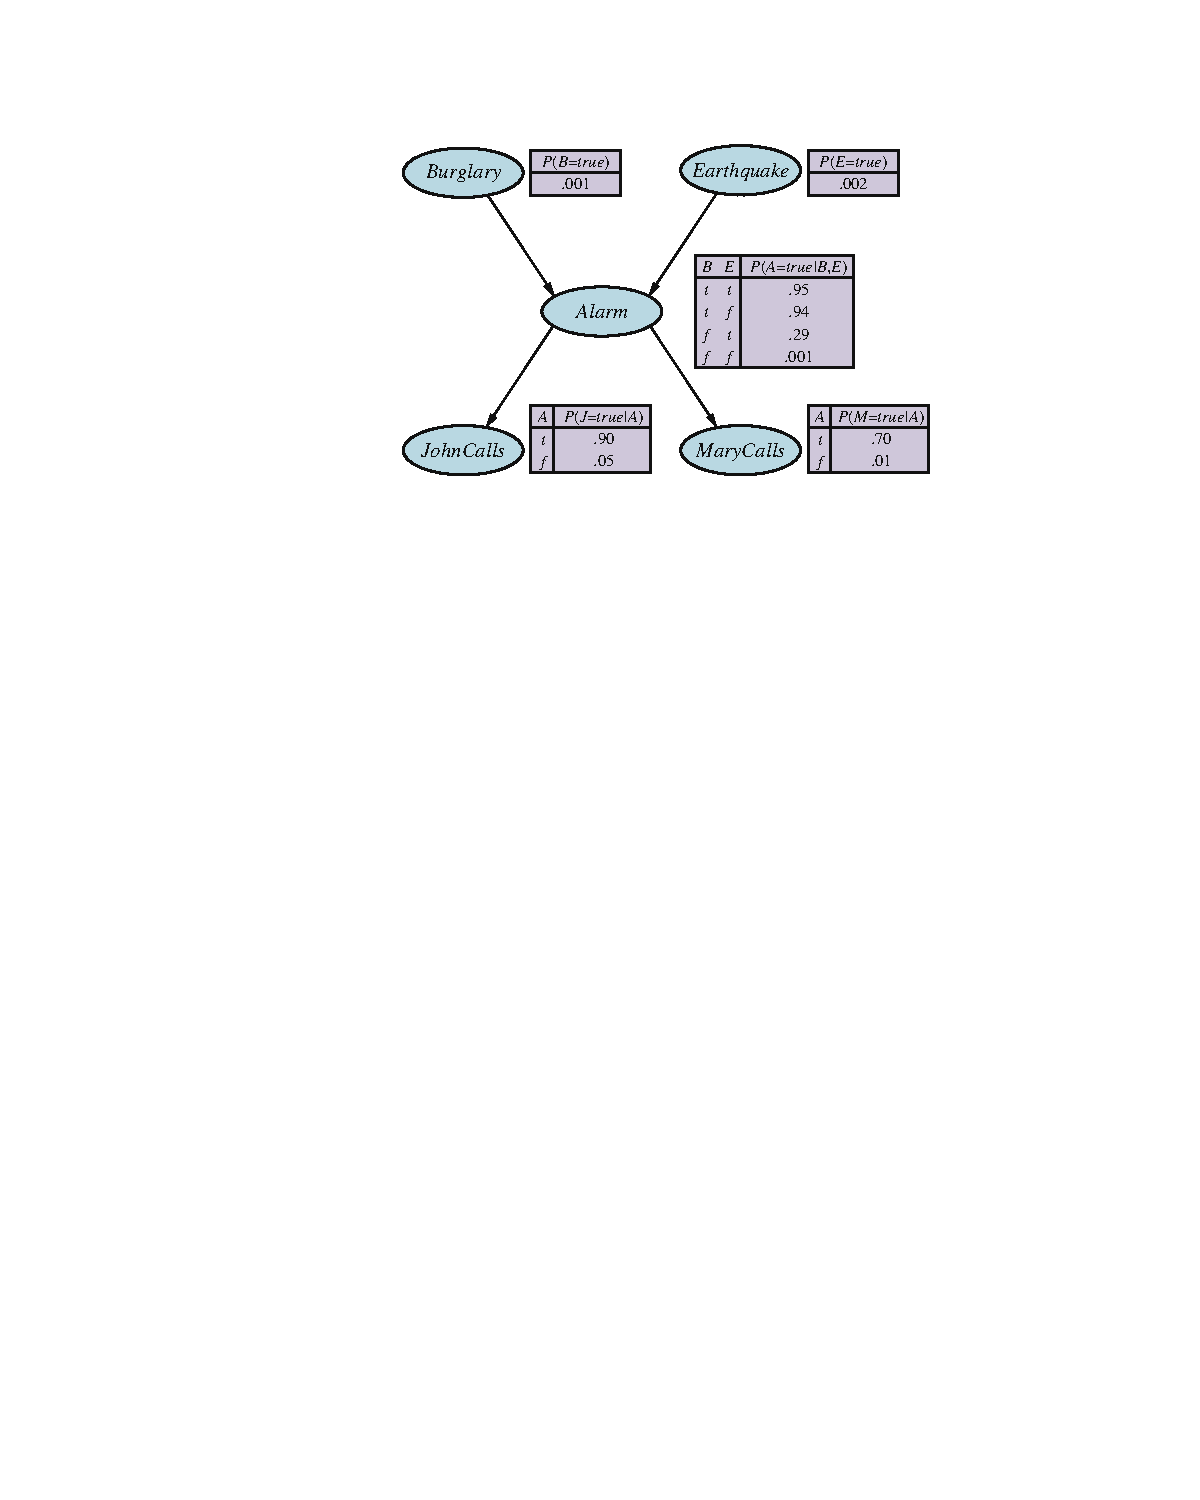
\includegraphics[alt={aima fig 13_02 bayes net alarm},width=0.75\linewidth]{aima-fig-13_02-bayes-net-alarm.pdf}


The full joint distribution for all the variables is defined by the topology and the
local probability information recorded in conditional probability tables (CPTs).
\section{Conditional Probability Tables}
\label{sec:org12e1dfe}

Each row in a CPT contains the conditional probability of each node value for a conditioning case.  A conditioning case is a possible combination of values for the parent nodes -- a miniature possible world.




\begin{itemize}
\item Each row must sum to 1, because the entries represent an exhaustive set of cases for the variable.

\item For Boolean variables, once you know the probability of \(true\) is \(p\), the probability of \(false\) must be \(1 - p\), so we often omit the second number.

\item In general, a table for a Boolean variable with \(k\) Boolean parents contains \(2^k\) independently specifiable probabilities.

\item A node with no parents has only one row, representing the prior probabilities of each possible value of the variable.
\end{itemize}





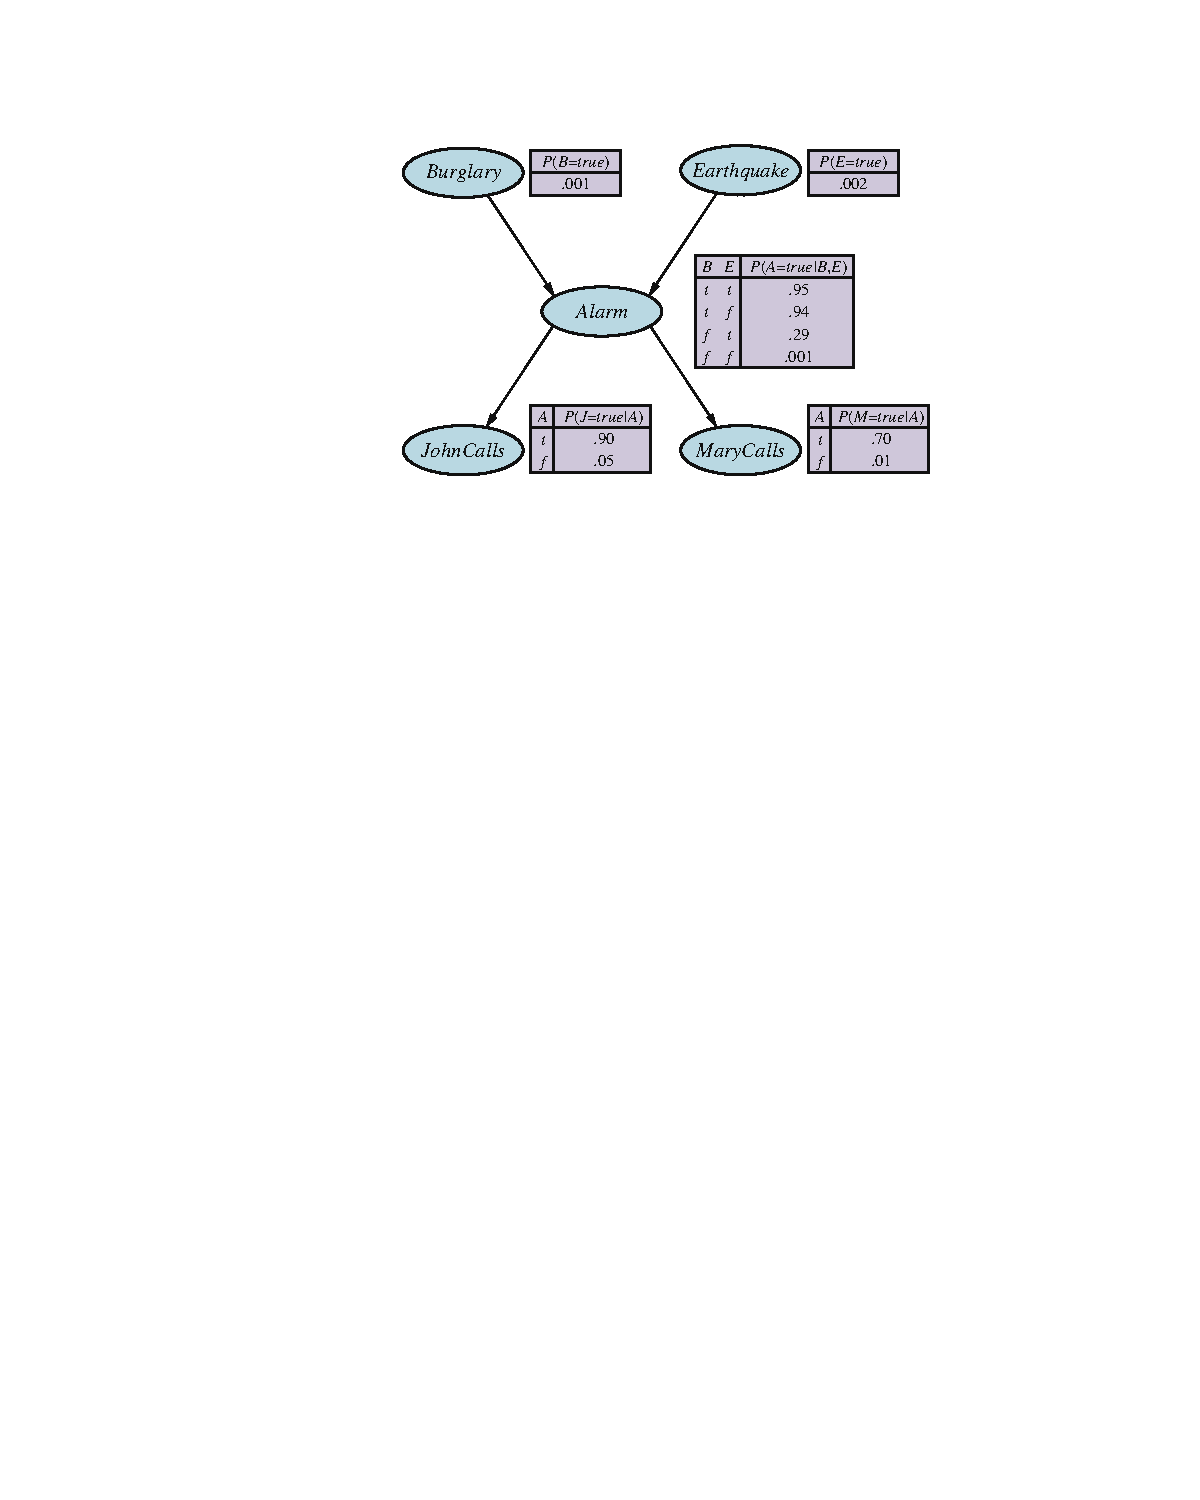
\includegraphics[alt={aima fig 13_02 bayes net alarm},width=0.75\linewidth]{aima-fig-13_02-bayes-net-alarm.pdf}
\section{Many Possibilities, Few Variables of Interest}
\label{sec:org56a78dd}

Network does not explicitly represent Mary currently listening to loud music or telephone ringing and confusing John.

\begin{itemize}
\item These factors are summarized in the uncertainty associated with the links from \(Alarm\) to \(JohnCalls\) and \(MaryCalls\).

\item This shows both laziness and ignorance in operation: a lot of work to find out the likelihood of those factors, and we have no reasonable way to obtain the relevant information anyway.
\end{itemize}

The probabilities actually summarize a potentially infinite set of circumstances:




\begin{itemize}
\item The alarm might fail to sound (humidity, power failure, dead battery, cut wires, a dead mouse stuck in the bell, etc.) or
\item John or Mary might fail to call and report it (out to lunch, on vacation, temporarily deaf, passing helicopter, etc.).
\end{itemize}





\includegraphics[alt={deadmau5},height=1in]{deadmau5.jpg}




In this way, a small agent can cope with a very large world, at least approximately.
\section{Semantics of Bayesian Networks}
\label{sec:org07a779b}

The \textbf{semantics} defines how the syntax -- a DAG with local probabilities -- corresponds to a joint distribution over the variables of the network.

A Bayes net contains:

\begin{itemize}
\item \(n\) variables, \(X_1, \dots , X_n\), and
\item (implicit) joint distributions \(P(X_1 = x_1 \land \dots \land X_n = x_n)\), or \(P(x_1, \dots, x_n)\).
\end{itemize}

Each entry in the joint distribution is defined by:

\begin{equation*}
P(x_1, \dots, x_n) = \prod_{i=1}^n \theta ( x_i | parents(X_i))
\end{equation*}

where \(parents(X_i)\) denotes the values of \(Parents(X_i)\) that appear in \(x_1, dots, x_n\).

So each entry in the joint distribution is the product of appropriate elements of the local CPTs in the Bayes net.
\section{Example: An Alarm, Two Calls, but No Events of Interest}
\label{sec:orgf21d0c9}




What is the probability that John and Mary call, but no earthquake or burglary occur?

\begin{itemize}
\item Take each entry \(i\) in each CPT \(\theta\) to mean \(P(x_1 | parents(X_i)\)

\begin{itemize}
\item The entries in the CPTs must be accurate conditional probabilities for the variables given their parents for the Bayes net to be useful in performing probabilistic inference.
\end{itemize}

\item Use those values in the calculation of the joint probability using
\end{itemize}
Using the abbreviations \(j, m, a, b\) and \(e\):





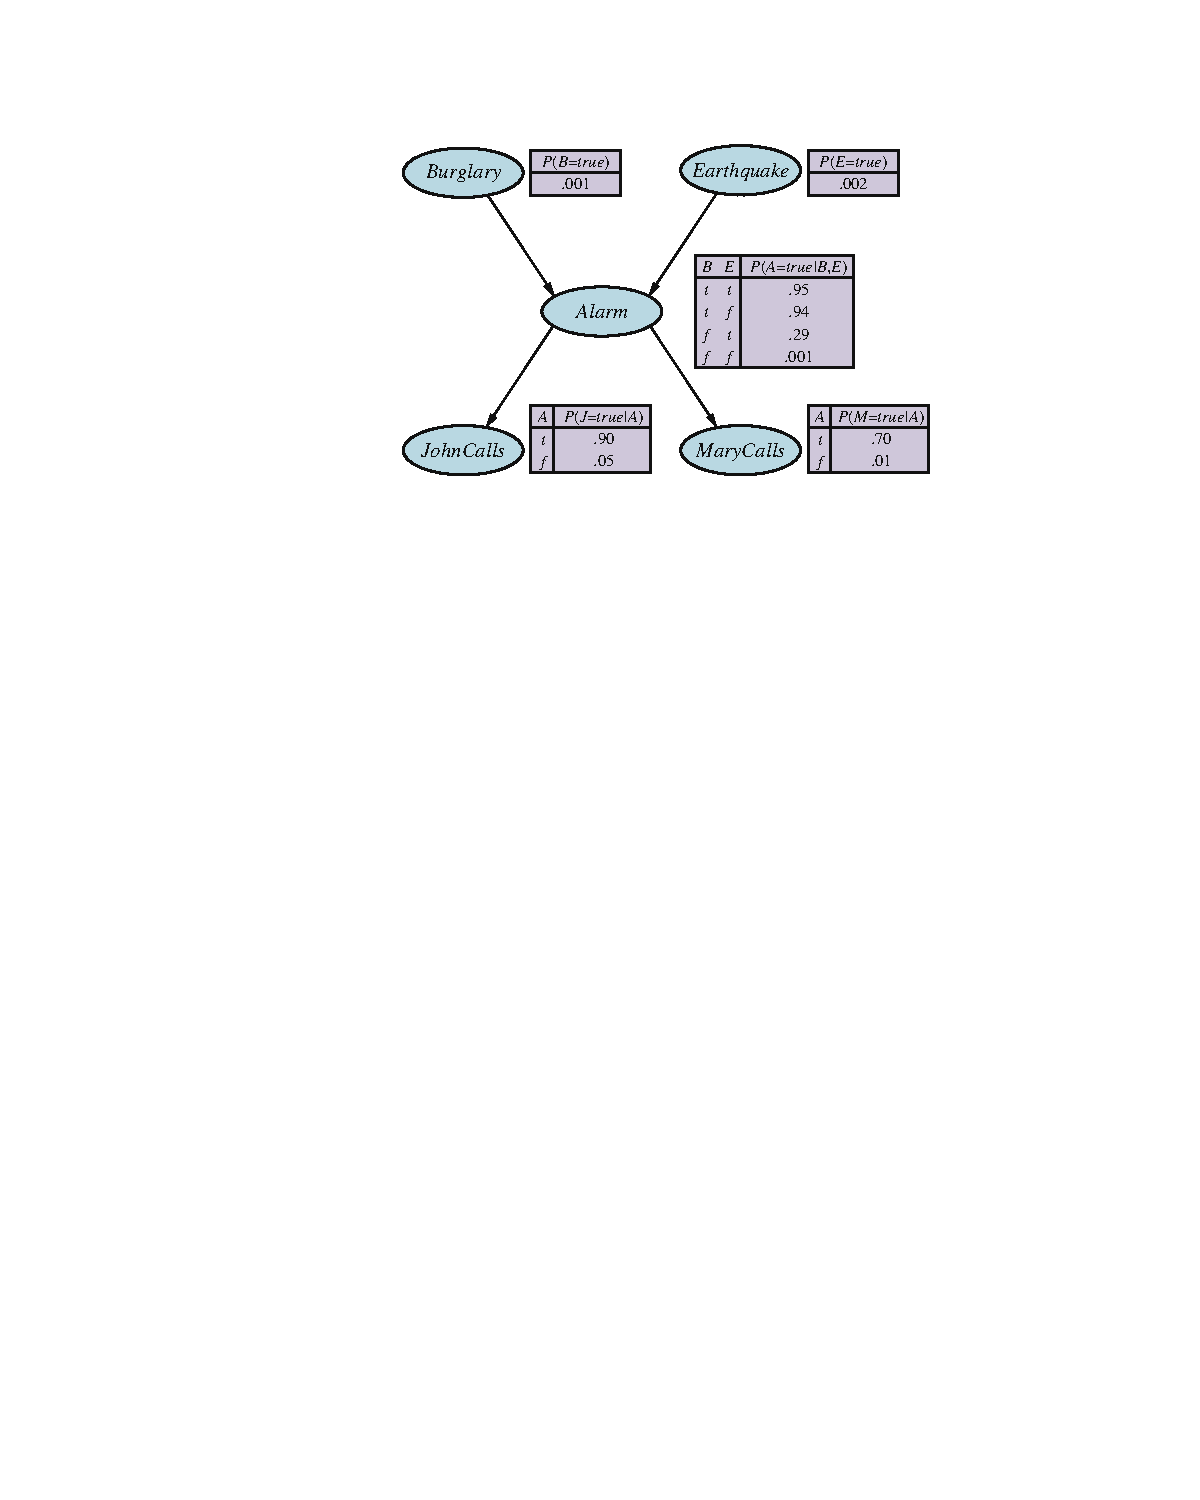
\includegraphics[alt={aima fig 13_02 bayes net alarm},height=1in]{aima-fig-13_02-bayes-net-alarm.pdf}





\begin{align*}
P(x_1, \dots, x_n)         &= \prod_{i=1}^n P( x_i | parents(X_i)) \tag{13.2}\\
P(j, m, a, \neg b, \neg e) &= P(j | a) P(m | a) P(a | \neg b, \neg e) P(\neg b) Pr (\neg e)\\
                            &= 0.90 \times 0.70 \times 0.001 \times 0.99 \times 0.98\\
                            &= 0.000628
\end{align*}
\section{Constructing Bayesian Networks}
\label{sec:org294ab73}

A Bayesian network is a correct representation of the domain only if each node is conditionally independent of its other predecessors in the node ordering, given its parents.  Mathematically, if \(Parents(X_i) \subseteq \{X_{i-1}, \dots, X_1\}\), then:

\begin{equation*}
P(X_i \mid X_{i-1}, \dots, X_i) = P(X_i \vert Parents(X_i)) \tag{13.3}
\end{equation*}

We can construct a valid Bayes net with this methodology:

\begin{enumerate}
\item Nodes: First determine the set of variables that are required to model the domain. Now order them, \(\{X_1, \dots ,X_n\}\). Any order will work, but the resulting network will be more compact if the variables are ordered such that causes precede effects.

\begin{itemize}
\item For the Burglary-Earthquake domain, \(B,E,A,J,M\) or \(E,B,A,M,J\) work.
\end{itemize}

\item Links: For \(i = 1\) to \(n\) do:

\begin{itemize}
\item Choose a minimal set of parents for \(X_i\) from \(X_1, \dots ,X_{i-1}\), such that Equation (13.3) is satisfied.
\item For each parent insert a link from the parent to \(X_i\).
\item CPTs: Write down the conditional probability table, \(P(X_i|Parents(X_i))\).
\end{itemize}
\end{enumerate}

Intuitively, the parents of node \(X_i\) should contain all those nodes in \(\{X_1,\dots,X_{i-1}\}\) that directly influence \(X_i\).
\section{Knowledge Engineering Considerations in Bayes Nets}
\label{sec:org1eedb00}




Suppose we have completed the network except for the choice of parents for \(MaryCalls\). We know:

\begin{itemize}
\item \(MaryCalls\) is influenced by  Burglary or Earthquake, but not directly. Our domain knowledge tells us that these events influence Mary’s calling behavior only through their effect on the alarm.
\item Also, given the state of the alarm, whether John calls has no influence on Mary’s calling.
\end{itemize}





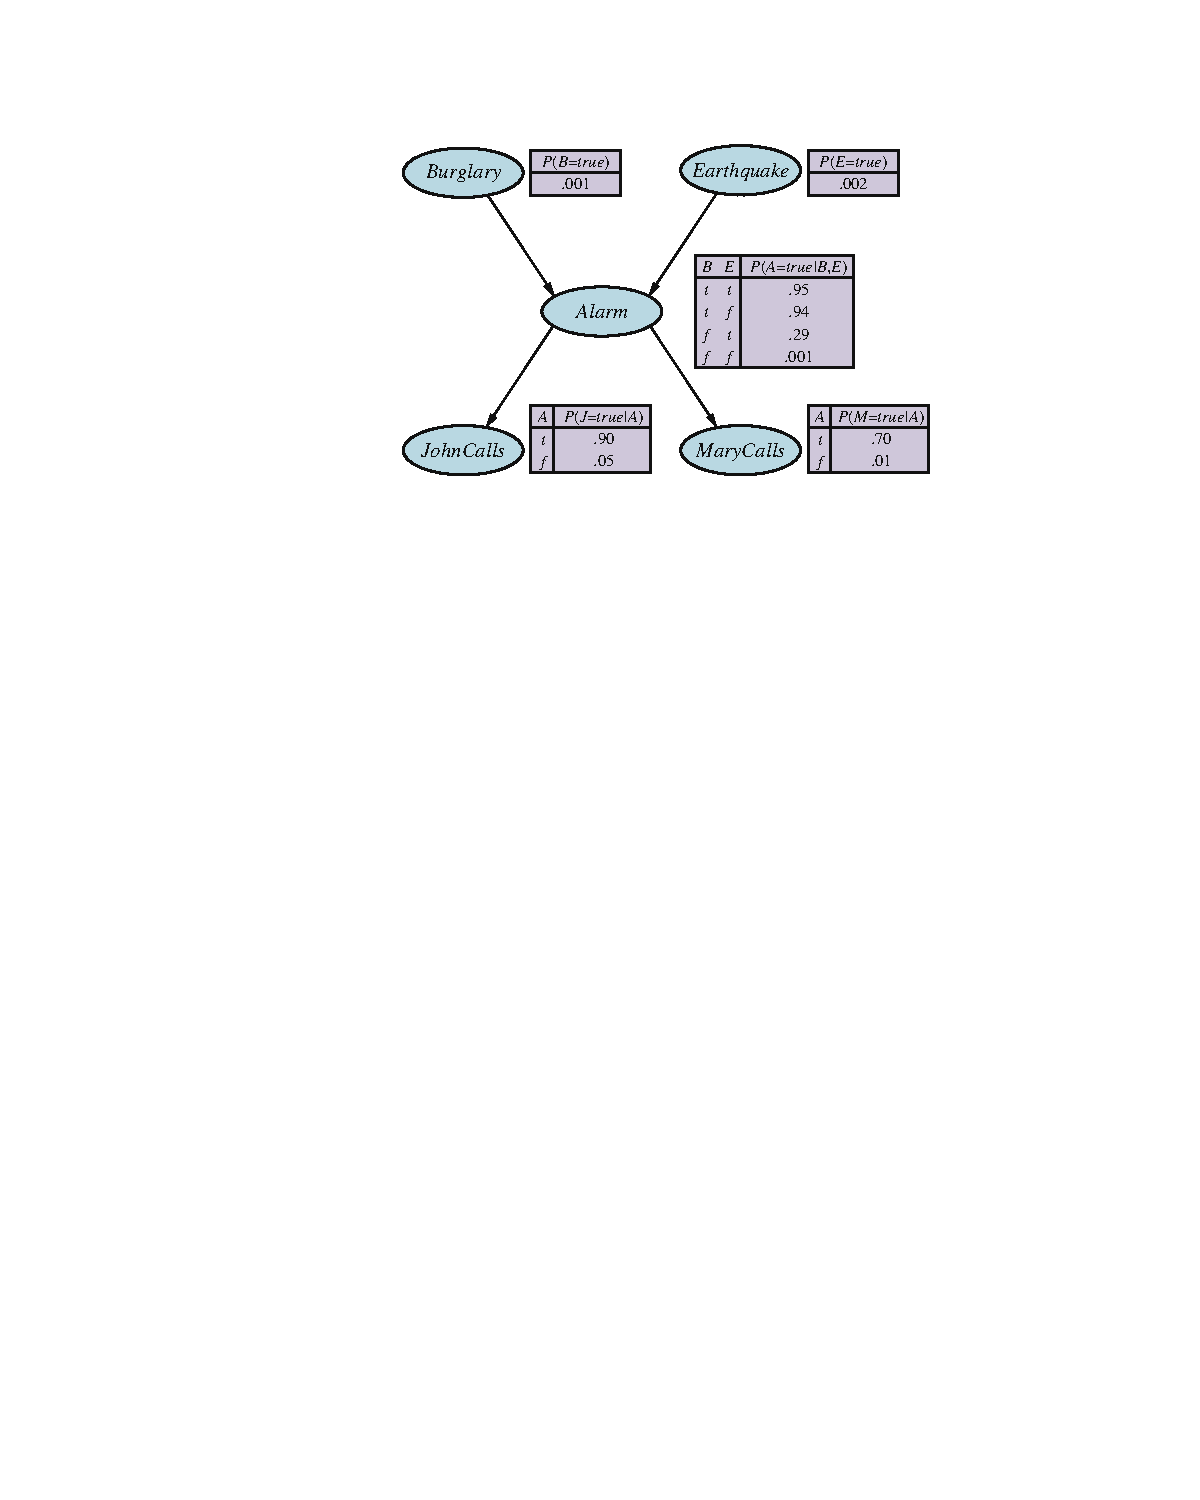
\includegraphics[alt={aima fig 13_02 bayes net alarm},height=1in]{aima-fig-13_02-bayes-net-alarm.pdf}





Formally, we believe that the following conditional independence statement holds:

\vspace{-.2in}
\[
P(MaryCalls \mid JohnCalls,Alarm,Earthquake,Burglary) = P(MaryCalls \mid Alarm).
\]
\vspace{-.2in}

Thus, Alarm will be the only parent node for MaryCalls.

Because

\begin{itemize}
\item each node is connected only to earlier nodes, this construction method guarantees that the network is acyclic, and
\item there are no redundant probability values,
\end{itemize}

there is no chance for inconsistency: it is impossible for the knowledge engineer or domain expert to create a Bayesian network that violates the axioms of probability.
\section{Compactness of Bayesian Network Models}
\label{sec:org3fae600}

Bayes nets are complete and nonredundant, but their \textbf{compactness} is their "secret sauce."

\begin{itemize}
\item Bayes nets are a kind of \textbf{locally structured}, or \textbf{sparse} system.

\begin{itemize}
\item In locally structured systems, each component interacts only with a bounded number, \(k\), of other components, where \(k \ll n\), the total number of components.
\item Local structure typically results in linear rather than exponential complexity.
\end{itemize}
\end{itemize}

Example: assume boolean variables.

\begin{itemize}
\item With \(n\) variables, the full joint distribution is \(2^n\) numbers.

\begin{itemize}
\item With 30 variables that's \(2^{30} = 1,073,741,824\) numbers.
\end{itemize}

\item With \(n\) variables, each of which is influenced by \(k\) parents, each CPT is \(2^k\) numbers and a full Bayesian network has \(n \cdot 2^k\) numbers.

\begin{itemize}
\item With 30 variables that's \(30 \cdot 2^5\) = 960 numbers.
\end{itemize}
\end{itemize}
\section{Effects of Node Ordering}
\label{sec:orgbd8e2b1}




We saw earlier that \(B, E, A, J, M\) is a good node ordering because causes come before effects.  With this node ordering we get 10 conditional probabilities.  What if we choose a different ordering, like \(M, J, A, B, E\)?

\begin{itemize}
\item Add \(MaryCalls\): No parents.

\item Add \(JohnCalls\): If Mary calls, alarm probably sounded, which increases prob that John calls.  So \(JohnCalls\) needs \(MaryCalls\) as a parent.

\item Add \(Alarm\): The more calls, the more likely alarm sounded, so \(Alarm\) needs \(MaryCalls\) and \(JohnCalls\) as parents.

\item Add \(Burglary\): Given knowledge of alarm, calls irrelevant: \(P(Burglary \mid Alarm,JohnCalls,MaryCalls) = P(Burglary \mid Alarm)\).  So just \(Alarm\) as parent.

\item Add \(Earthquake\): With alarm, earthquake more likely.  But burglary explains alarm, and probability of an earthquake only slightly higher than normal. So need both \(Alarm\) and \(Burglary\) as parents.
\end{itemize}

We end up with 13 conditional probabilities.





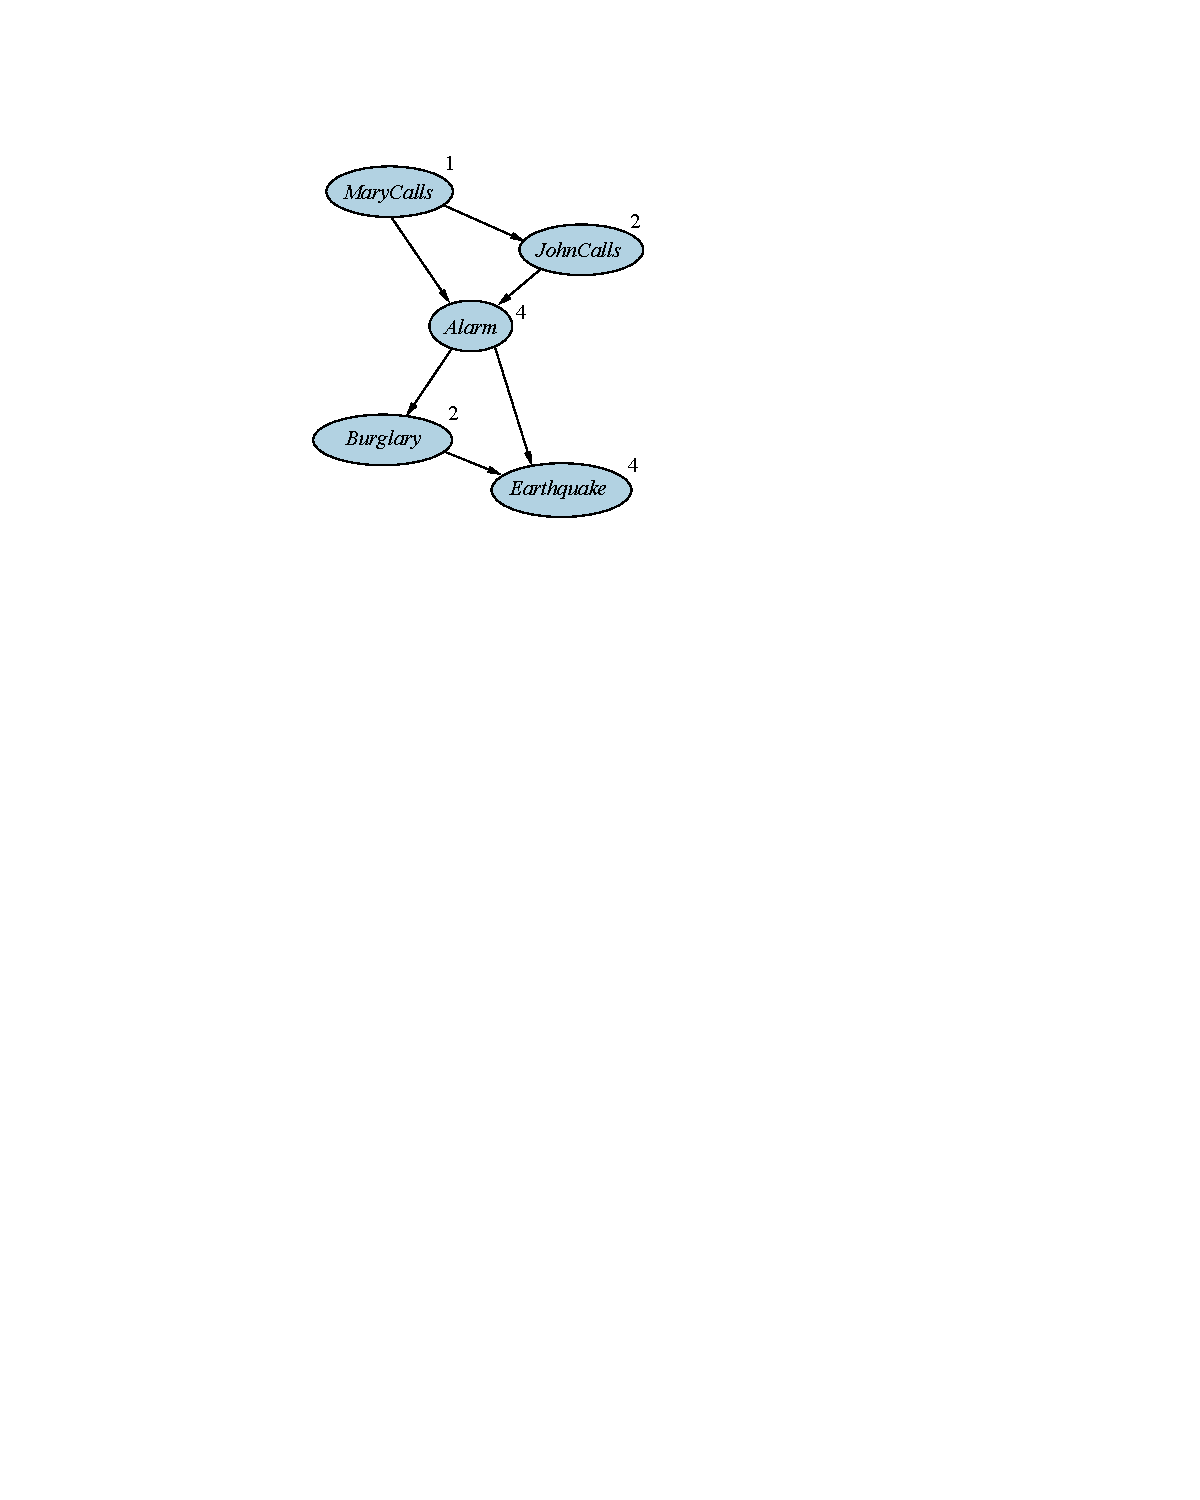
\includegraphics[alt={aima fig 13_03_a bayes net mjabe ordering},width=0.75\linewidth]{aima-fig-13_03_a-bayes-net-mjabe-ordering.pdf}
\section{Knowledge Engineering in Probabilistic Systems}
\label{sec:orgc9a7cd8}





There is still knowledge engineering involved, which includes design choices.

\begin{itemize}
\item You may choose to trade a small amount of accuracy for the improved performance of leaving out an influence variable.

\begin{itemize}
\item If there's a large earthquake, John and Mary probably won't call even if they hear the alarm.  Could choose to include links from \(EarthQuake\) to \(JohnCalls\) and \(MaryCalls\).  This would increase accuracy slightly, but probably not worth the extra complexity.
\end{itemize}

\item And as we just saw, node ordering matters, potentially quite a bit.

\begin{itemize}
\item With node ordering \(M, J, E, B, A\) the resulting Bayes net requires 31 probabilities -- same as the full joint distribution.
\end{itemize}
\end{itemize}





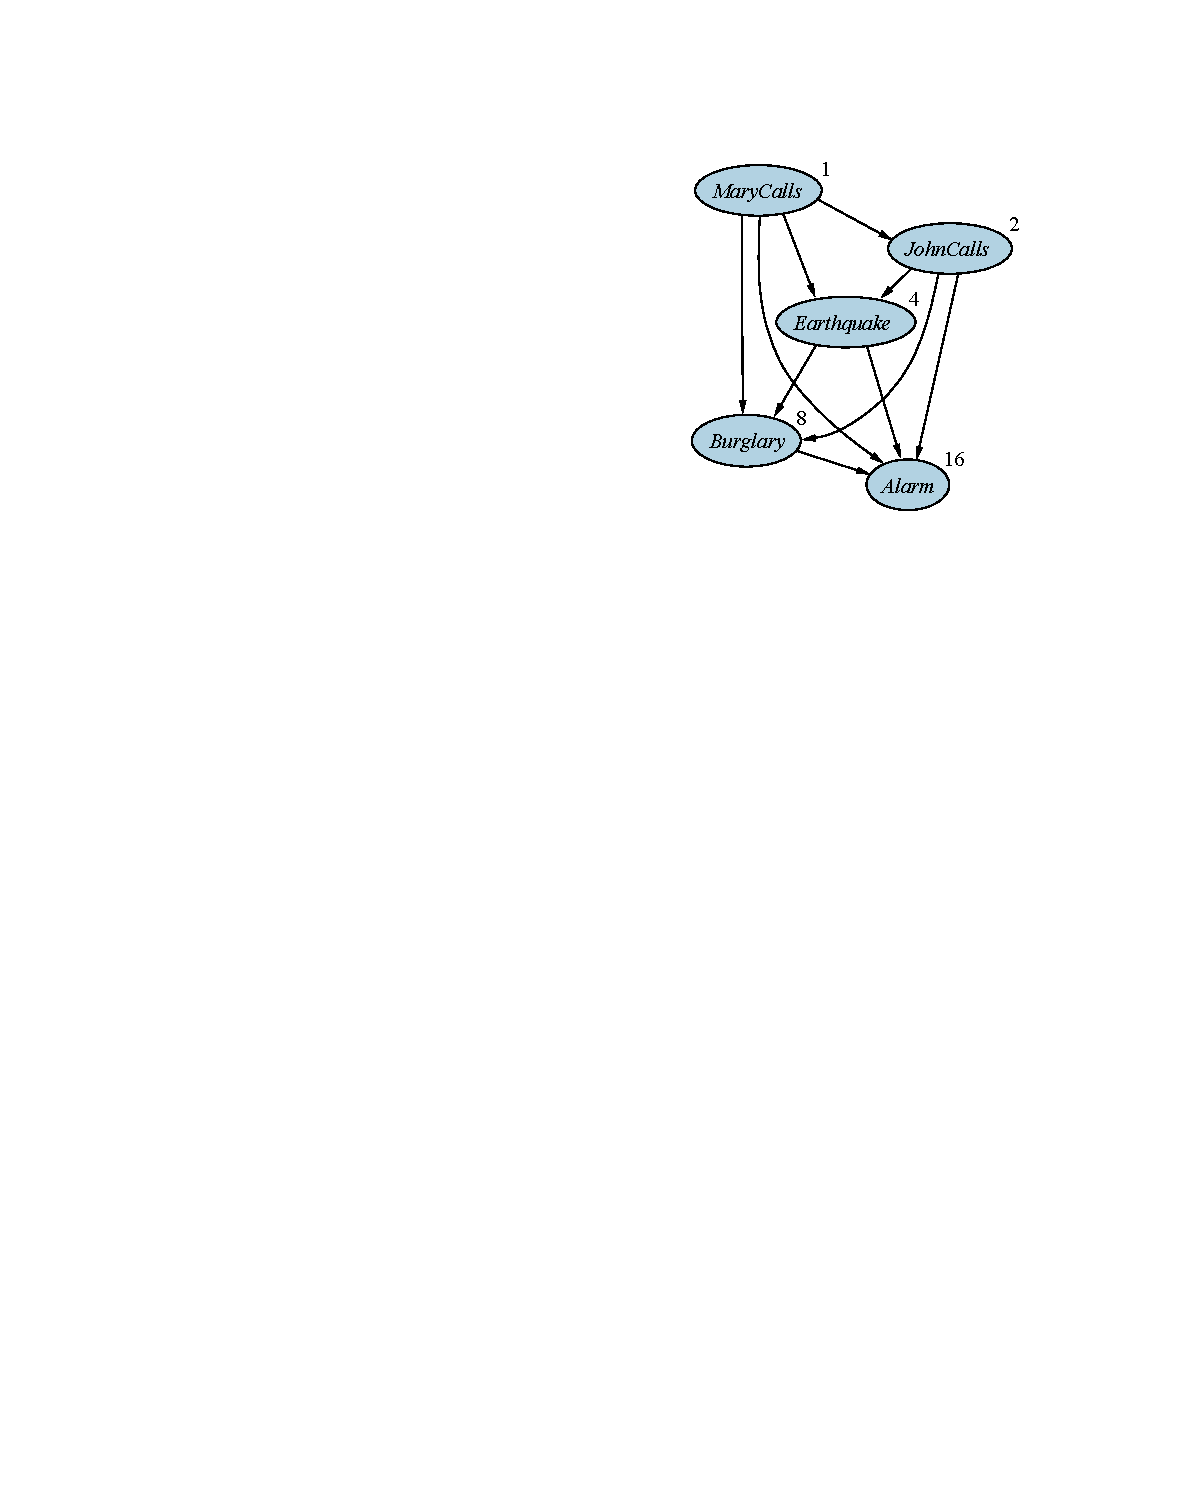
\includegraphics[alt={aima fig 13_03_b bayes net mjeba ordering},height=1in]{aima-fig-13_03_b-bayes-net-mjeba-ordering.pdf}





Any Bayes net represents the same joint distibution, but some are far more efficient.

\begin{quote}
Key takeaway: stick to causal models.  They are easier to specify, easier to get right, and they lead to more efficient Bayes nets.
\end{quote}
\section{Exact Inference in Bayesian Networks (AIMA 13.3)}
\label{sec:org06ba8b5}

Most common task in probabilistic inference: compute the \textbf{posterior probability} of a set of \textbf{query variables} given some \textbf{event} represented as a set of \textbf{evidence variables}.




Notation:

\begin{itemize}
\item Query variable: \(X\)
\item Set of evidence variables: \(\bm{E} = \{E_1, \dots, E_m\}\)
\item Particular observed event: \(\bm{e}\)
\item Hidden (nonevidence, nonquery) variables: \(\bm{Y} = \{Y_1, \dots, Y_l\}\)
\item Typical query: \(P(X \mid e)\)
\end{itemize}

Example:

\begin{itemize}
\item \(X\) is the boolean random variable \(Burglary\)
\item \(\bm{E} = \{JohnCalls, MaryCalls\}\)
\item \(\bm{e} = \{JohnCalls = true, MaryCalls = true\}\)
\item \(\bm{Y} = \{EarthQuake, Alarm\}\)
\end{itemize}






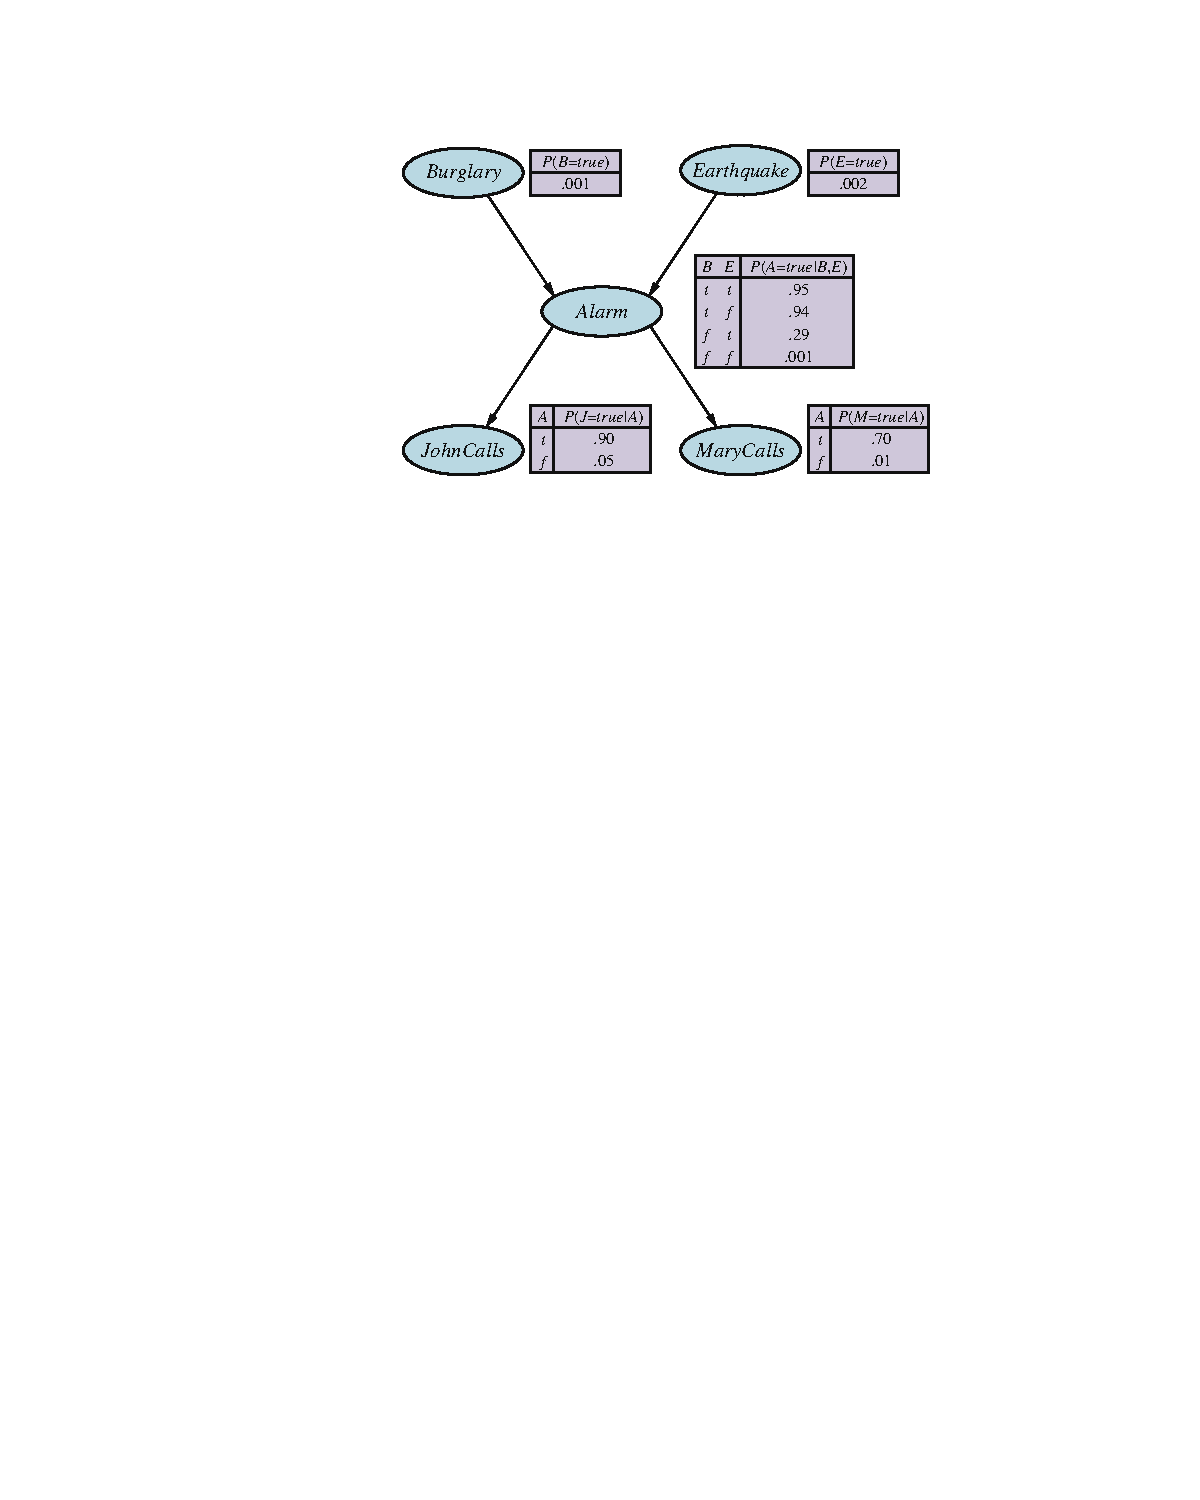
\includegraphics[alt={aima fig 13_02 bayes net alarm},width=0.75\linewidth]{aima-fig-13_02-bayes-net-alarm.pdf}





\begin{equation*}
P(Buglary \mid JohnCalls = true, MaryCalls = true) = <0.284, 0.716>.
\end{equation*}
\section{Inference by Enumeration}
\label{sec:org884871e}

Recall that we can use the full joint distribution to answer any query:

\begin{equation*}
P(X \mid \bm{e})
= \frac{P(\bm{e} \mid X) P(X)}{P(\bm{e})}
= \frac{P(\bm{e}, X)}{P(\bm{e})}
= \frac{P(X, \bm{e})}{P(\bm{e})}
= \alpha P(X, \bm{e})
= \alpha \sum_y P(X, \bm{e}, \bm{y}) \tag{12.9}
\end{equation*}


And that a Bayes net completely represents the full joint distribution, so we can reduce the computation of a joint to:

\begin{equation*}
P(x_1, \dots, x_n) = \prod_{i=1}^n P( x_i | parents(X_i)) \tag{13.2}
\end{equation*}

Using these two equations we can enumerate the appropriate probabilities to calculate the answer to any probabilistic query.

\begin{itemize}
\item In particular, we can get the answer by computing sums of products of conditional probabilities from a Bayes net.
\end{itemize}
\section{Example: Prob of Burglary Given JohnCalls = true and MaryCalls = true.}
\label{sec:org63c7832}

Using abbreviations and substituting into Eq 12.9 above (\(e\) and \(a\) are hidden):

\[
P(B \mid j, m) = \alpha P(B, j, m) = \alpha \sum_e \sum_a P(B, j, m, e, a)
\]

Then we substitute Eq 13.2 for \(P(B, j, m, e, a)\) to get (only showing Burglary=true by the notation \(b\)):

\vspace{-.1in}
\begin{align*}
P(b \mid j, m) &= \alpha \sum_e \sum_a P(b) P(e) P(a \mid b, e) P(j \mid a) P(m \mid a) \tag{1}\\
                &= \alpha P(b) \sum_e \sum_a P(e) P(a \mid b, e) P(j \mid a) P(m \mid a) \tag{2}\\
                &= \alpha P(b) \sum_e P(e) \sum_a P(a \mid b, e) P(j \mid a) P(m \mid a) \tag{3}
\end{align*}
\vspace{-.1in}

\begin{enumerate}
\item Substitute Eq 13.2 for \(P(B, j, m, e, a)\)
\item Pull out \(P(b)\) from summations because it doesn't depend on the other variable and is thus a constant in all the summation terms.
\item Pull out \(P(e)\) from the summation over the \(a\) values because each value of \(e\) doesn't depend on the other variables in the summation over the \(a\) values and is thus a constant in the summation terms over the values of \(a\).
\end{enumerate}

Steps 2 and 3 above reduce the complexity of the computation from \(O(n2^n)\) to \(O(2^n)\).
\section{Caclulation of Burglary given John and Mary Call}
\label{sec:org439ea69}




Substiting the values from the CPTs in the Bayes net into
\begin{equation*}
\alpha P(b) \sum_e P(e) \sum_a P(a \mid b, e) P(j \mid a) P(m \mid a)
\end{equation*}

we get the expression tree:


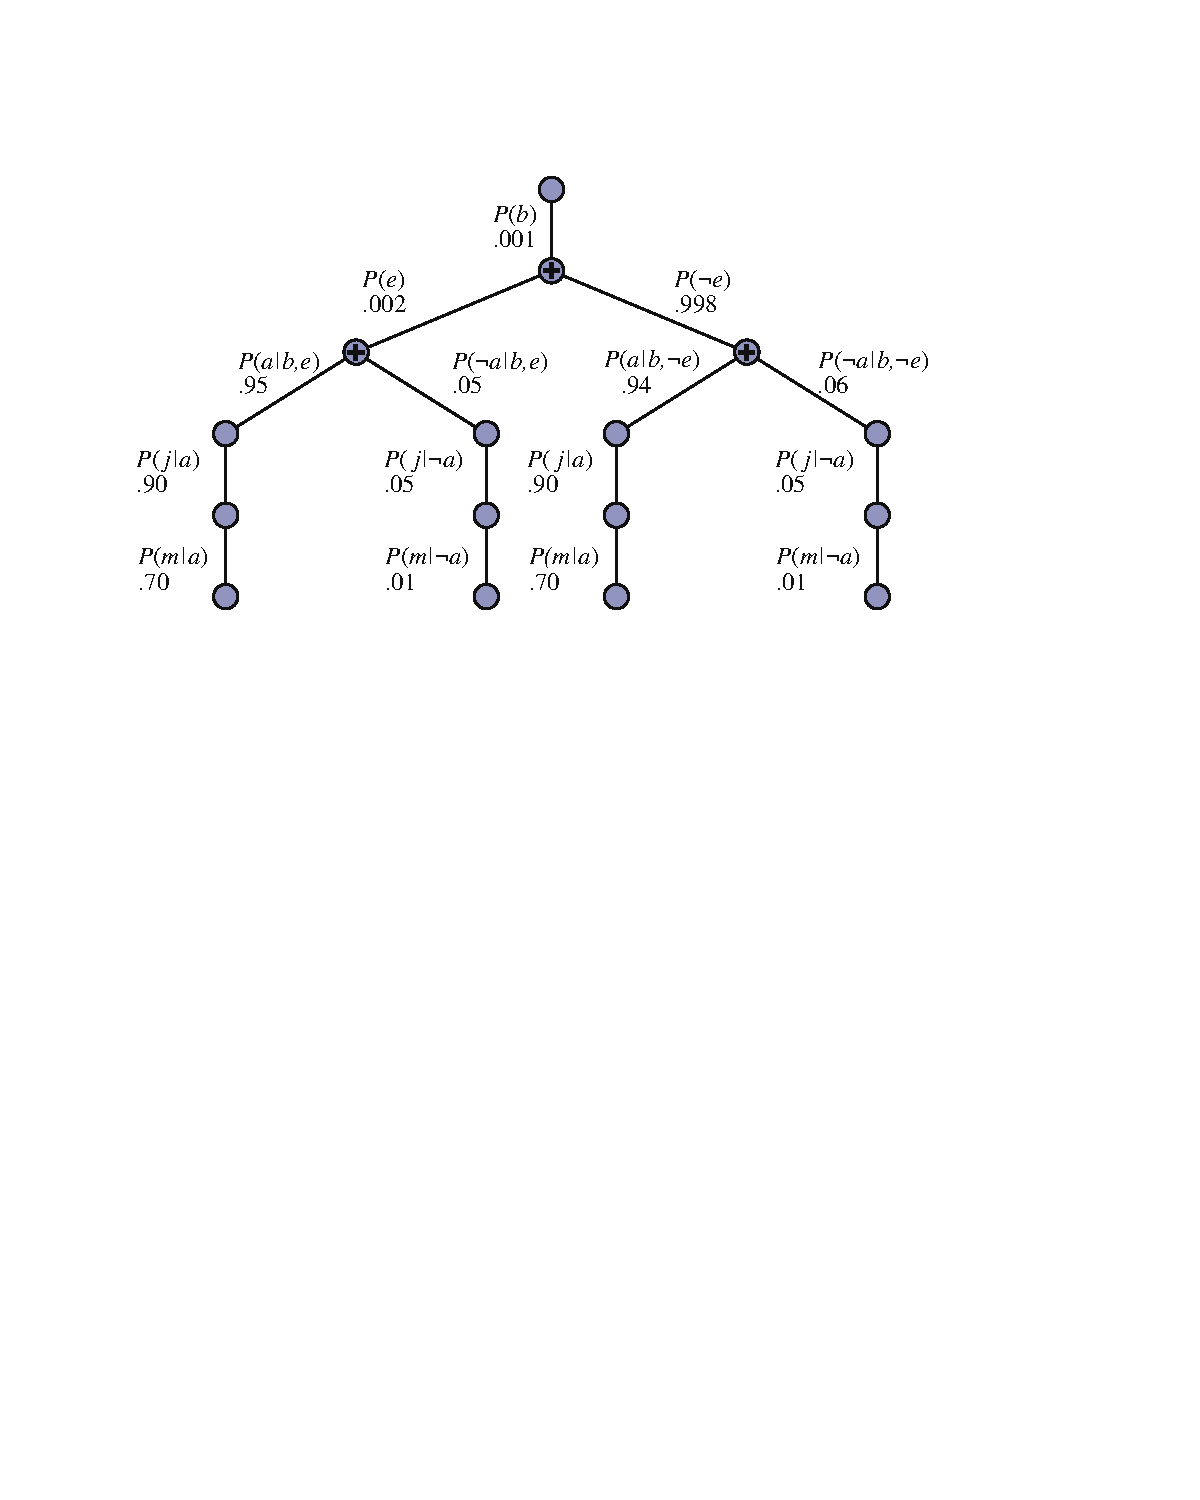
\includegraphics[alt={aima fig 13_10 prob expression tree},height=1in]{aima-fig-13_10-prob-expression-tree.pdf}







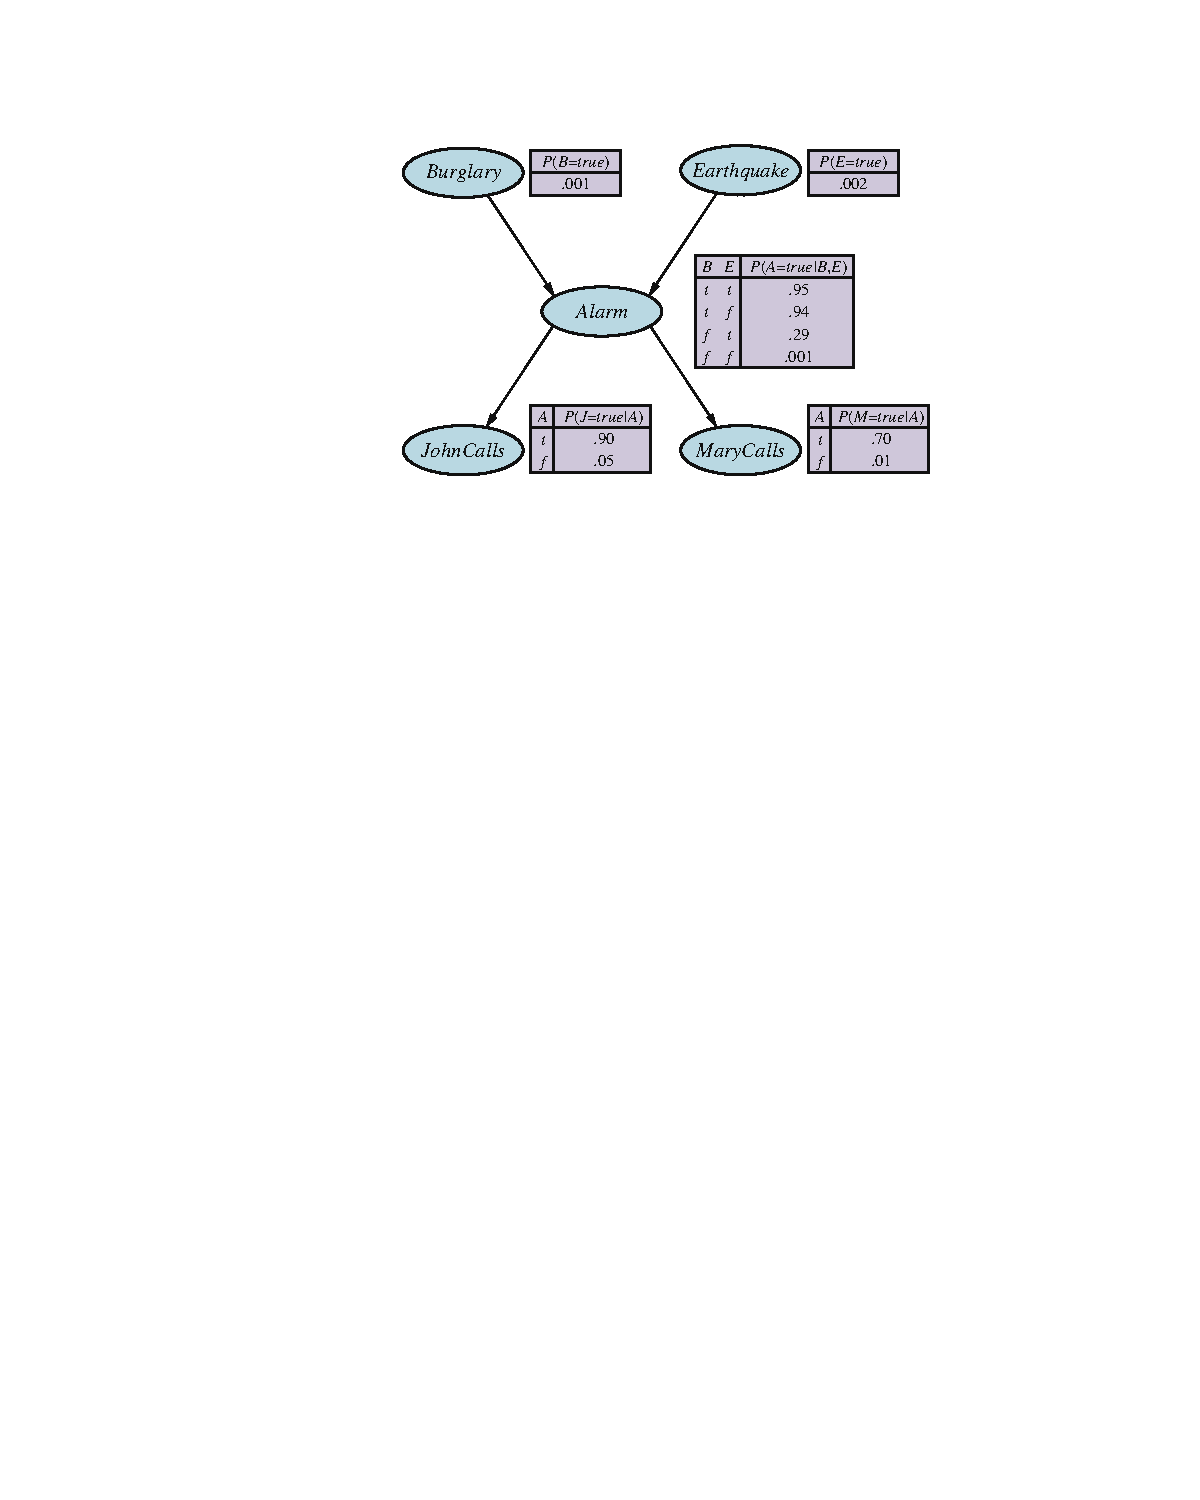
\includegraphics[alt={aima fig 13_02 bayes net alarm},height=1in]{aima-fig-13_02-bayes-net-alarm.pdf}
\section{Enumeration Algorithm}
\label{sec:org0a97e9d}

The ENUMERATION-ASK algorithm evaluates these expression trees using depth-first, left-to-right recursion.


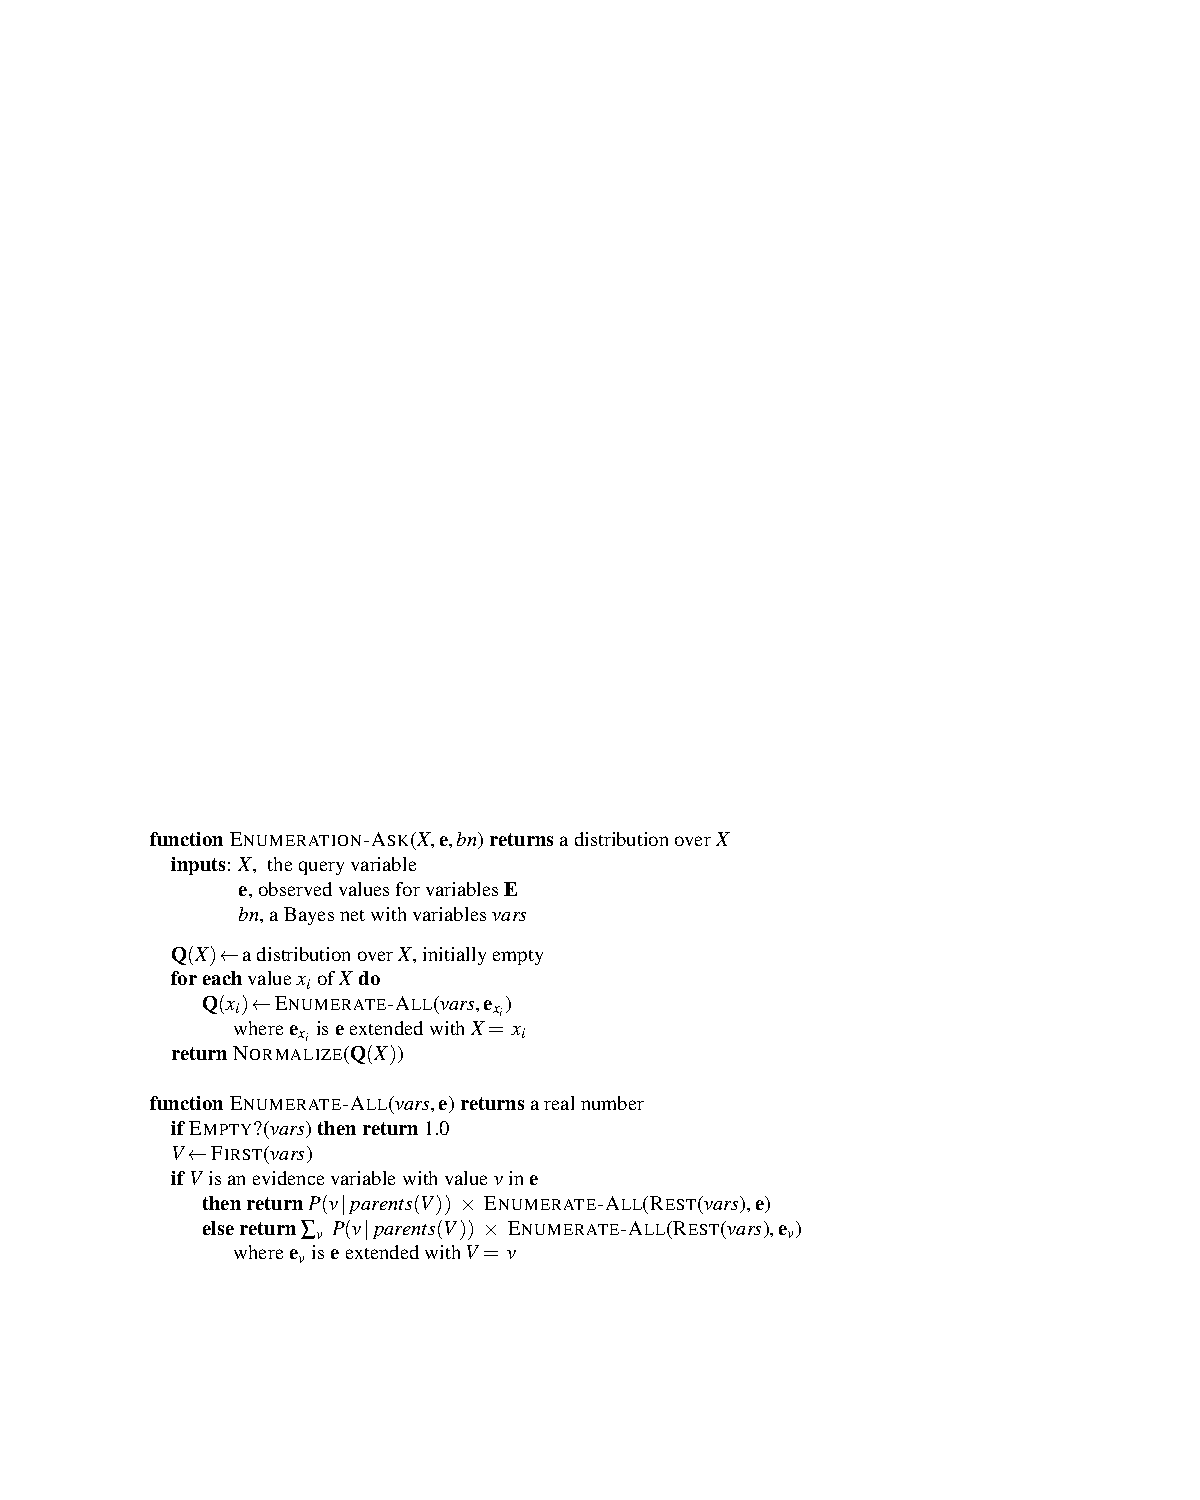
\includegraphics[alt={aima fig 13_11 bayes net enumeration algorithm},width=0.75\linewidth]{aima-fig-13_11-bayes-net-enumeration-algorithm.pdf}


Unfortunately, its time complexity is \(O(s^n)\).  But we can improve it \ldots{}
\section{Repeated Calculations}
\label{sec:org7e627a8}

Notice that the subexpressions for the products \(P(j \mid a) P(m \mid a)\) and \(P(j \mid \neg a) P(m \mid \neg a)\) are computed twice, once for each value of \(E\).


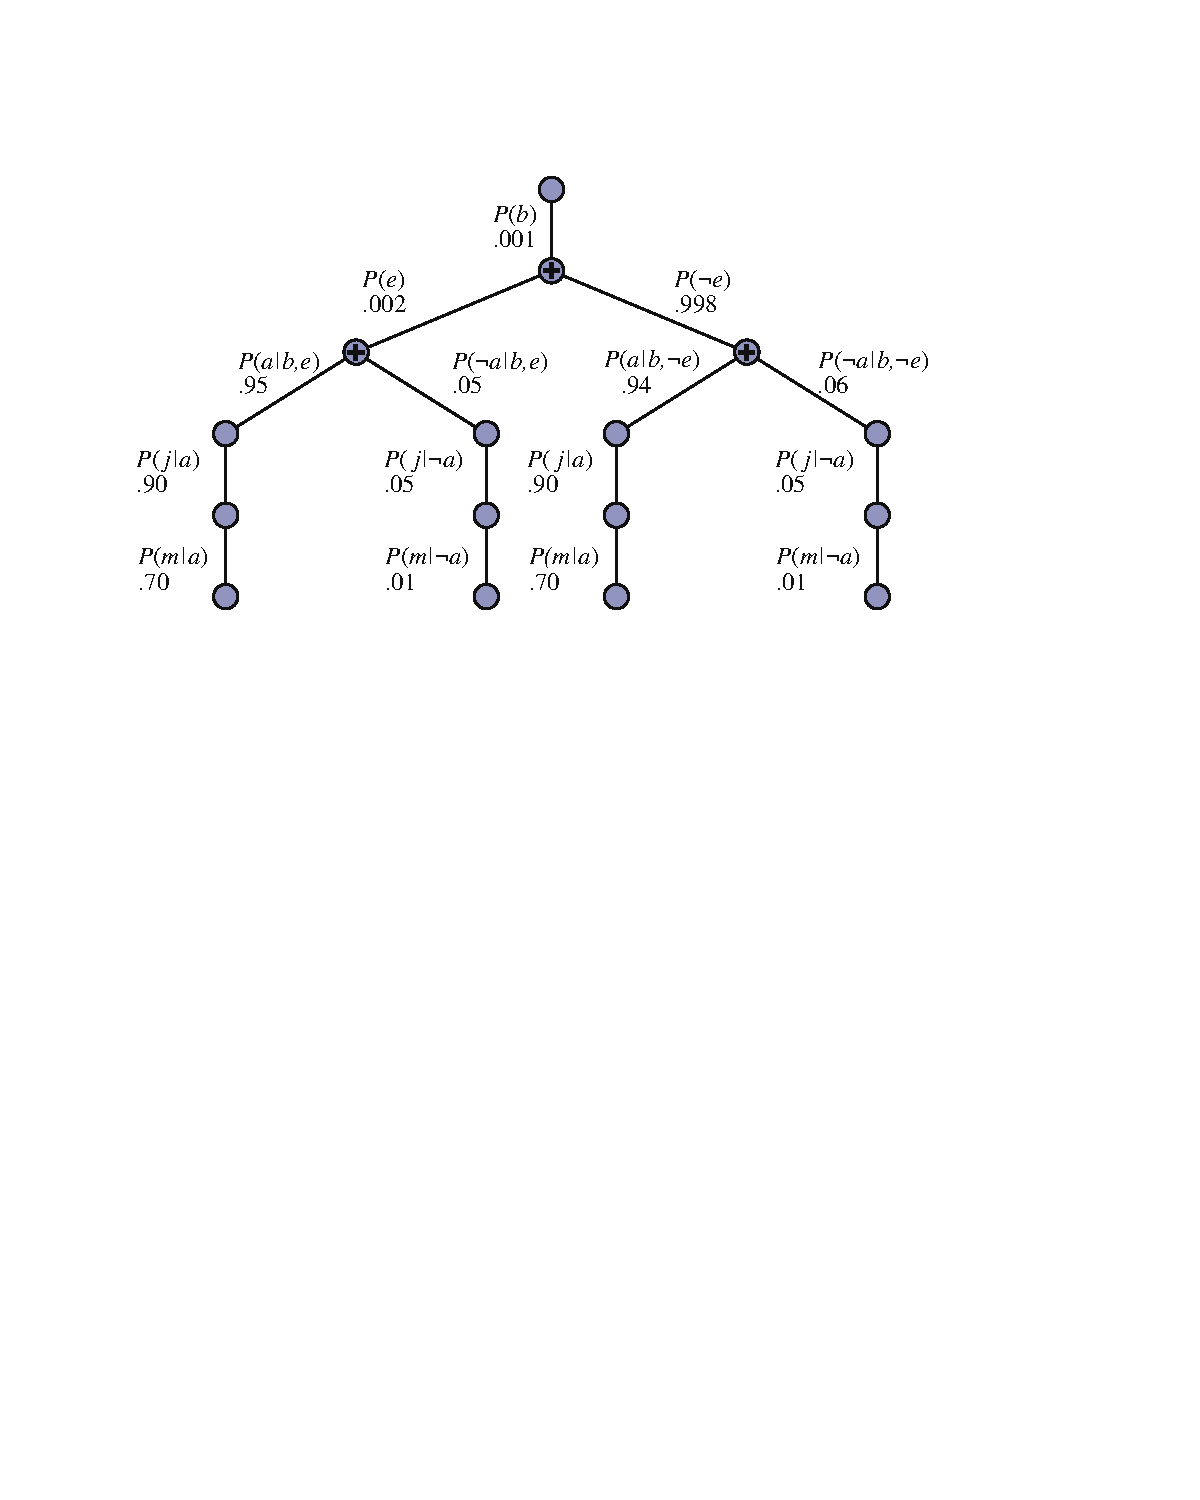
\includegraphics[alt={aima fig 13_10 prob expression tree},width=0.75\linewidth]{aima-fig-13_10-prob-expression-tree.pdf}
\section{Variable Elimination}
\label{sec:orge3a6aff}

The enumeration algorithm can be improved substantially by eliminating repeated calculations.

\begin{itemize}
\item Idea:  do the calculation once and save the results for later use.
\item This is a form of dynamic programming.
\item Several versions of this approach; variable elimination algorithm is simplest.
\end{itemize}

Variable elimination works by evaluating expressions such as

\begin{equation*}
P(b \mid j, m) = \alpha P(b) \sum_e P(e) \sum_a P(a \mid b, e) P(j \mid a) P(m \mid a) \tag{13.5}
\end{equation*}

in right-to-left order (that is, bottom up in the expression tree), storing intermediate results, and only doing summations for portions of the expression that depend on the variable.
\section{Example: Variable Elimination in Burglary Network}
\label{sec:org30f8274}

First, annotate the *factor*s in the expression for the network:

\begin{equation*}
P(B \mid j, m) =
\alpha \underbrace{P(B)}_{\bm{f}_1(B)}
\sum_e
\underbrace{P(e)}_{\bm{f}_2(E)}
\sum_a
\underbrace{P(a \mid B, e)}_{\bm{f}_3(A,B,E)}
\underbrace{P(j \mid a)}_{\bm{f}_4(A)}
\underbrace{P(m \mid a)}_{\bm{f}_5(A)}
\end{equation*}

\begin{itemize}
\item Each factor is a matrix indexed by the values of its argument variables.
\item Notice that the factors for \(P(j \mid a)\) and \(P(m | a)\) do not include \(j\) and \(m\).  This is because the values of \(j\) and \(m\) (\(JohnCalls=true\) and \(MaryCalls-true\)) are fixed by the query.
\end{itemize}

So the factors are:




\begin{equation*}
\bm{f}_1(B) =
\begin{bmatrix}
P(b) \\
P(\neg b)
\end{bmatrix}
=
\begin{bmatrix}
0.001 \\
0.999
\end{bmatrix}
\end{equation*}




\begin{equation*}
\bm{f}_2(E) =
\begin{bmatrix}
P(e) \\
P(\neg e)
\end{bmatrix}
=
\begin{bmatrix}
0.002 \\
0.998
\end{bmatrix}
\end{equation*}




\vspace{.2in}




\begin{equation*}
\bm{f}_4(A) =
\begin{bmatrix}
P(j \mid a) \\
P(j \mid \neg a)
\end{bmatrix}
=
\begin{bmatrix}
0.090 \\
0.05
\end{bmatrix}
\end{equation*}




\begin{equation*}
\bm{f}_5(A) =
\begin{bmatrix}
P(m \mid a) \\
P(m \mid \neg a)
\end{bmatrix}
=
\begin{bmatrix}
0.070 \\
0.01
\end{bmatrix}
\end{equation*}





\vspace{.2in}

\(\bm{f}_3(A, B, E)\) is a little more complicated \ldots{}
\section{Calculation of F 3}
\label{sec:org35a2bab}

\begin{equation*}
P(B \mid j, m) =
\alpha \underbrace{P(B)}_{\bm{f}_1(B)}
\sum_e
\underbrace{P(e)}_{\bm{f}_2(E)}
\sum_a
\underbrace{P(a \mid B, e)}_{\bm{f}_3(A,B,E)}
\underbrace{P(j \mid a)}_{\bm{f}_4(A)}
\underbrace{P(m \mid a)}_{\bm{f}_5(A)}
\end{equation*}

\(\bm{f}_3(A, B, E)\) is a \(2 \times 2 \times 2\) matrix (or a rank-3 tensor).  Here's one way to think about it:

\begin{itemize}
\item First index with \(A\), yielding two \(2 \times 2\) submatrices (one for each of the two values of \(A\)).
\item Rows of each submatrix is indexed by \(B\) and columns by \(E\).
\item The entries in the submatrices are the values of \(P(A \mid B, E)\)
\end{itemize}



\begin{equation*}
\bm{f}_{3}^{(a)} (B, E) =
\begin{bmatrix}
P(a \mid b,e) & P(a \mid b, \neg e) \\
P(a \mid \neg b, e) & P(a \mid \neg b, \neg e)
\end{bmatrix}
=
\begin{bmatrix}
0.95 & 0.94\\
0.29 & 0.001
\end{bmatrix}
\end{equation*}

\begin{equation*}
\bm{f}_{3}^{(\neg a)} (B, E) =
\begin{bmatrix}
P(\neg a \mid b,e) & P(\neg a \mid b, \neg e) \\
P(\neg a \mid \neg b, e) & P(\neg a \mid \neg b, \neg e)
\end{bmatrix}
=
\begin{bmatrix}
0.05 & 0.06\\
0.71 & 0.999
\end{bmatrix}
\end{equation*}




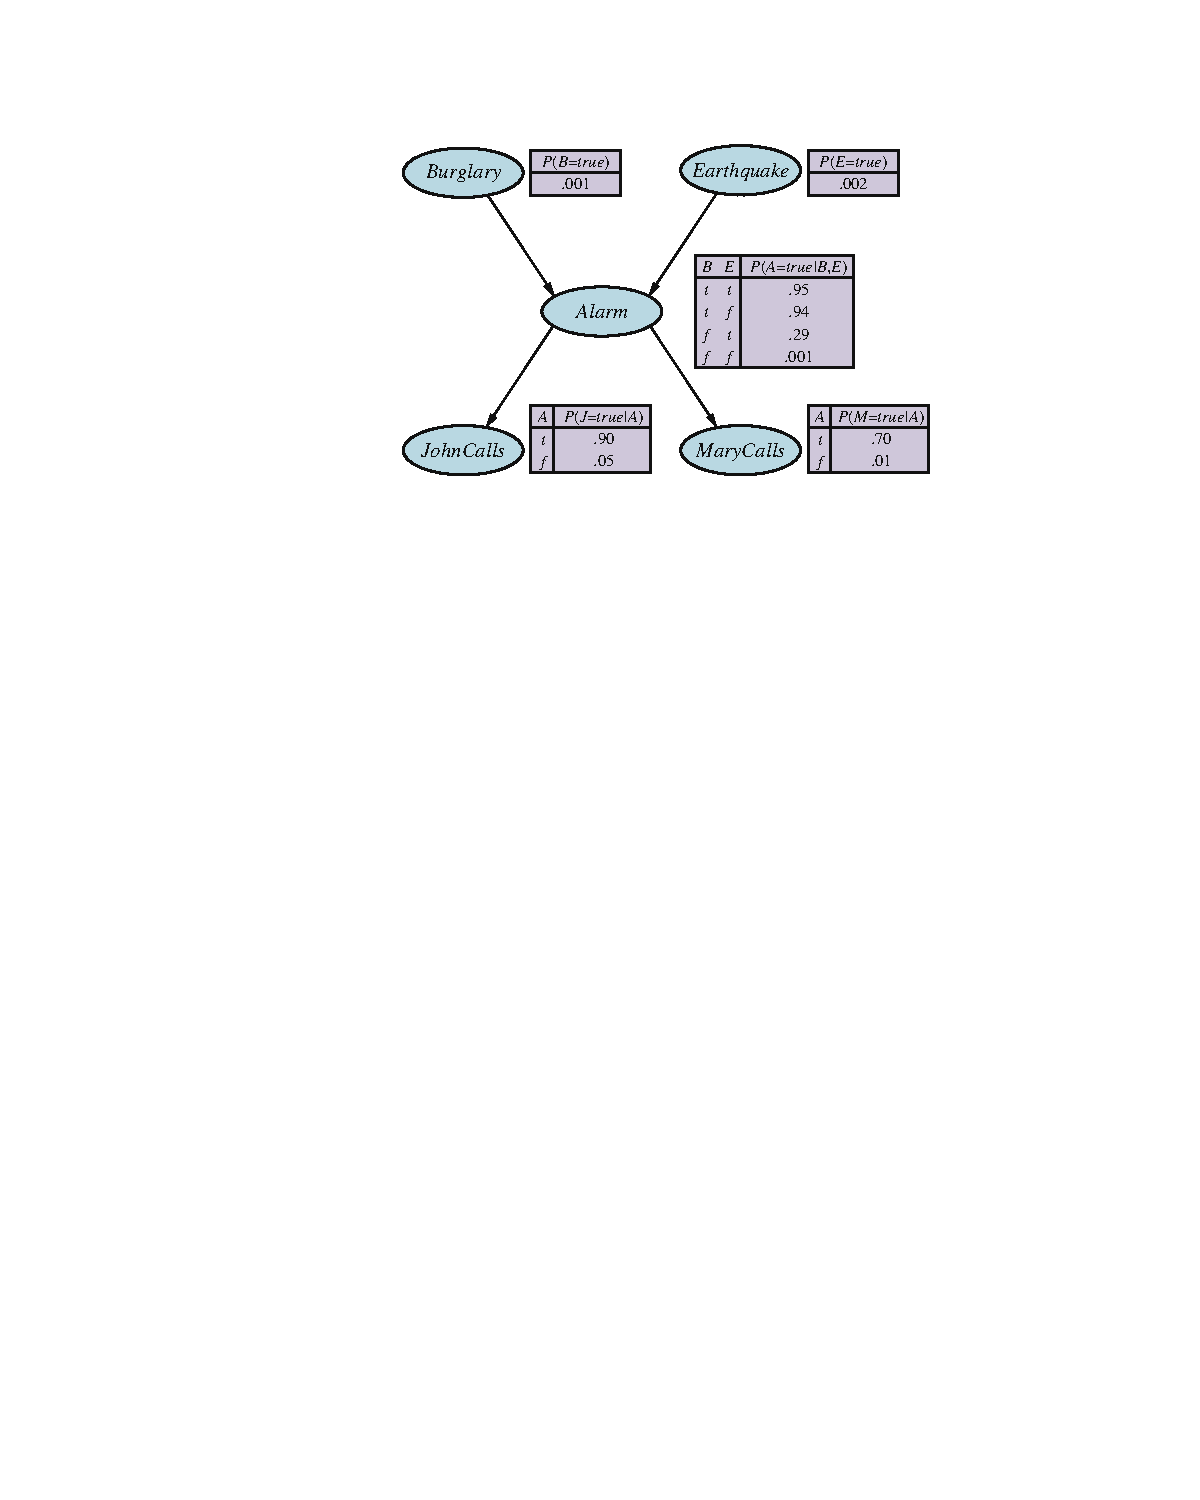
\includegraphics[width=0.75\textwidth, right]{aima-fig-13_02-bayes-net-alarm.pdf}
\section{Factorized Query}
\label{sec:org4f9d684}

From our original query:

\begin{equation*}
P(b \mid j, m) = \alpha P(b) \sum_e P(e) \sum_a P(a \mid b, e) P(j \mid a) P(m \mid a) \tag{13.5}
\end{equation*}

We annotated the factors:


\begin{equation*}
P(B \mid j, m) =
\alpha \underbrace{P(B)}_{\bm{f}_1(B)}
\sum_e
\underbrace{P(e)}_{\bm{f}_2(E)}
\sum_a
\underbrace{P(a \mid B, e)}_{\bm{f}_3(A,B,E)}
\underbrace{P(j \mid a)}_{\bm{f}_4(A)}
\underbrace{P(m \mid a)}_{\bm{f}_5(A)}
\end{equation*}

And now we substitute the factor expressions for the original expresions so we can manipulate the factors using the \textbf{pointwise product} operation, denoted with \(\times\) here:

\begin{equation*}
P(B \mid j, m) =
\alpha \bm{f}_1(B) \times \sum_e \bm{f}_2(E) \times \sum_a \bm{f}_3(A,B,E) \times \bm{f}_4(A) \times \bm{f}_5(A)
\end{equation*}

Now we are ready to evaluate the expression \ldots{}
\section{Expression Evaluation}
\label{sec:orgbfda973}

Given our factorized query:

\vspace{-.1in}
\[
P(B \mid j, m) =
\alpha \bm{f}_1(B) \times \sum_e \bm{f}_2(E) \times \sum_a \bm{f}_3(A,B,E) \times \bm{f}_4(A) \times \bm{f}_5(A)
\]

First, sum out A from the pointwise product of \(\bm{f}_3(A,B,E)\), \(\bm{f}_4(A)\), and \(\bm{f}_5(A)\) yielding a new \(2 \times 2\) factor, \(\bm{f}_6(B,E)\):

\vspace{-.2in}
\begin{align*}
\bm{f}_6(B,E) &= \sum_a \bm{f}_3(A,B,E) \times \bm{f}_4(A) \times \bm{f}_5(A) \\
              &= (\bm{f}_3(a,B,E) \times \bm{f}_4(a) \times \bm{f}_5(a)) + (\bm{f}_3(\neg a,B,E) \times \bm{f}_4(\neg a) \times \bm{f}_5(\neg a))
\end{align*}
\vspace{-.2in}

Now the query expression is \(P(B \mid j, m) =
\alpha \bm{f}_1(B) \times \sum_e \bm{f}_2(E) \times \bm{f}_6 (B, E)\)

Next, sum out \(E\) from the product of \(\bm{f}_2 (E)\) and \(\bm{f}_6 (B, E)\), yielding a new factor \(\bm{f}_7 (B)\):

\vspace{-.2in}
\begin{align*}
\bm{f}_7(B) &= \sum_e \bm{f}_2(E) \times \bm{f}_6(B, E) \\
            &= \bm{f}_2(e) \times \bm{f}_6(B, e) + \bm{f}_2(\neg e) \times \bm{f}_6(B, \neg e)
\end{align*}
\vspace{-.1in}

Which leaves our final form of the query: \(P(B \mid j, m) =\alpha \bm{f}_1(B) \times \bm{f}_7(B)\)

This expression can be evaluated by taking the pointwise product and normalizing the result.
\section{Operations on Factors}
\label{sec:orgf49135c}

In the preceding manipulations we saw the two basic operations in variable elimination:

\begin{enumerate}
\item the pointwise product operation, and
\item summing out hidden variables from products of factors.
\end{enumerate}

Now let's see how we calculate them.
\section{Pointwise Product Example}
\label{sec:org4c8e325}

The pointwise product of two factors \(\bm{f}\) and \(\bm{g}\) yields a new factor \(\bm{h}\) whose variables are the union of the variables in \(\bm{f}\) and \(\bm{g}\) and whose elements are given by the product of the corresponding elements in the two factors.

Given \(X, Y, Z\) boolean variables, result of pointwise product \(\bm{f}(X, Y) \times \bm{g}(Y, Z) = \bm{h}(X, Y, Z)\) is:


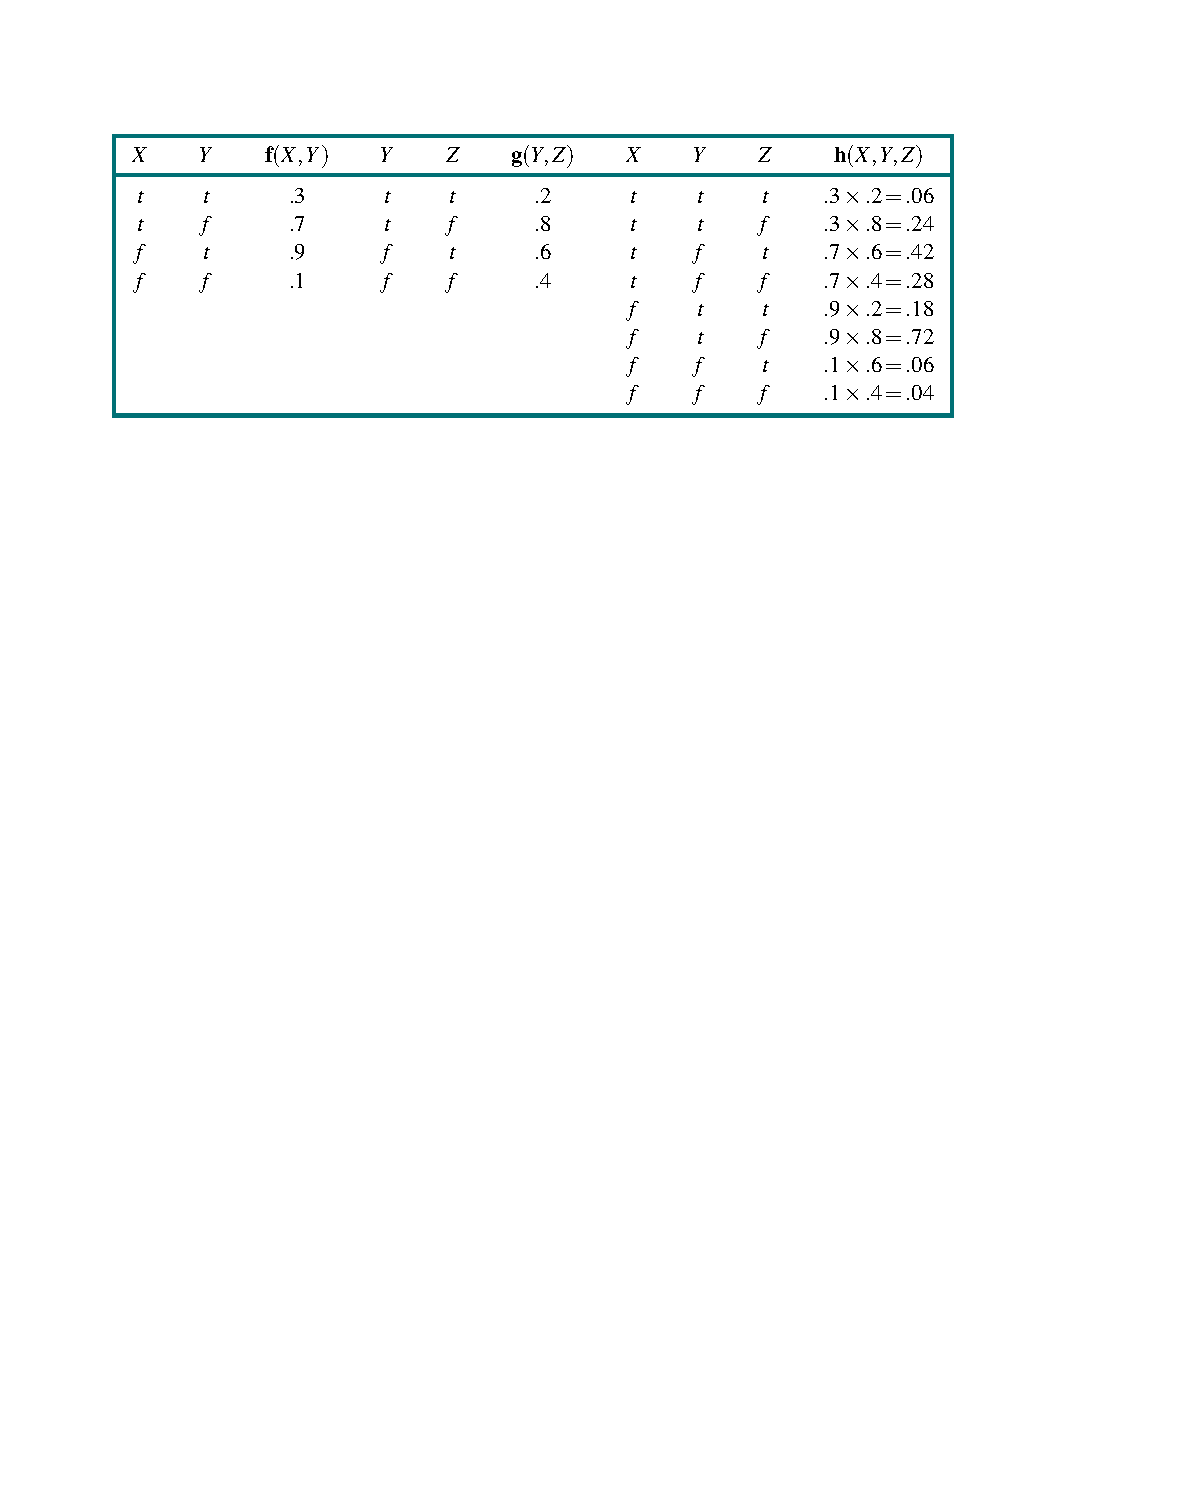
\includegraphics[alt={aima fig 13_12 pointwise multiplication},height=1in]{aima-fig-13_12-pointwise-multiplication.pdf}
\section{Summing out Variables}
\label{sec:org0b16f6e}



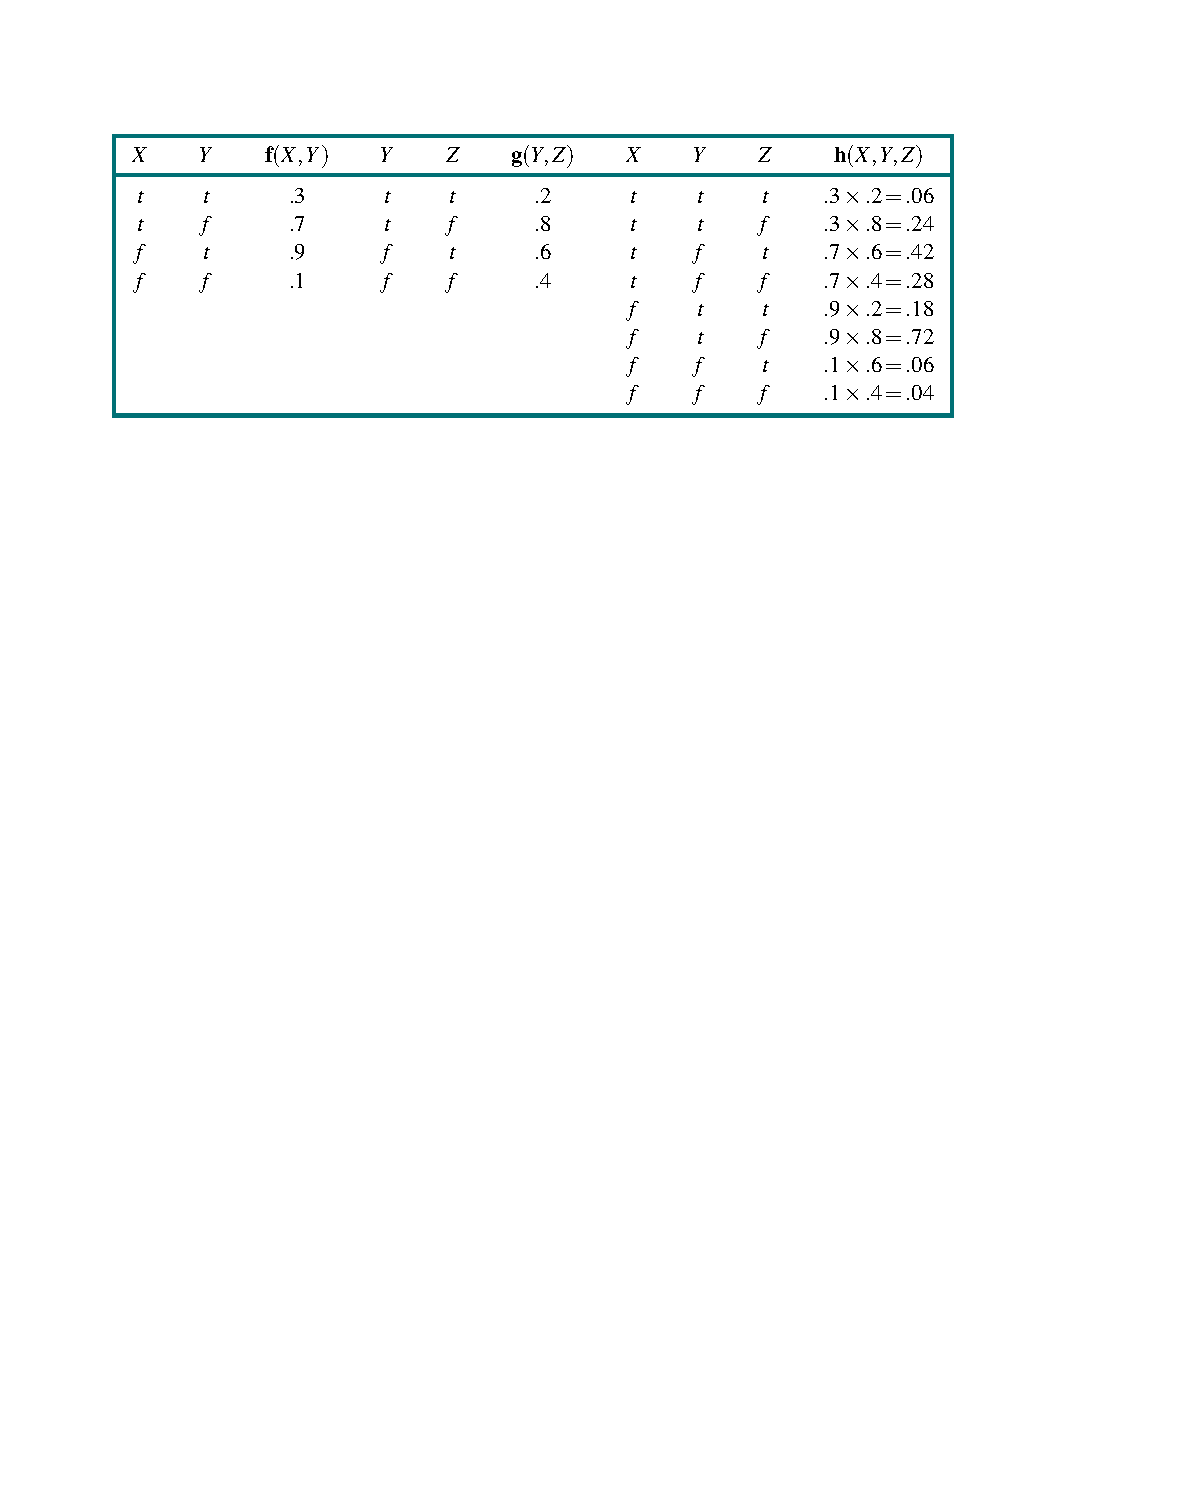
\includegraphics[alt={aima fig 13_12 pointwise multiplication},height=1in]{aima-fig-13_12-pointwise-multiplication.pdf}



Summing out a variable from a product of factors is done by adding up the submatrices
formed by fixing the variable to each of its values in turn. For example, to sum out \(X\) from
\(h(X,Y,Z)\), we write

\vspace{-.25in}
\begin{align*}
\bm{h}_2 (Y, Z) &= \sum_x \bm{h}(X, Y, Z)\\
                &= \bm{h}(x, Y, Z) + \bm{h}(\neg x, Y, Z) \\
&=
\begin{bmatrix}
.06 & .24 \\
.42 & .28
\end{bmatrix}
+
\begin{bmatrix}
.18 & .72 \\
.06 & .04
\end{bmatrix} \\
&=
\begin{bmatrix}
.24 & .96 \\
.48 & .32
\end{bmatrix}
\end{align*}
\section{Variable Elimination Algorithm}
\label{sec:orgafb99ed}

With these two basic operations, we can implement the variable elimination algorithm:


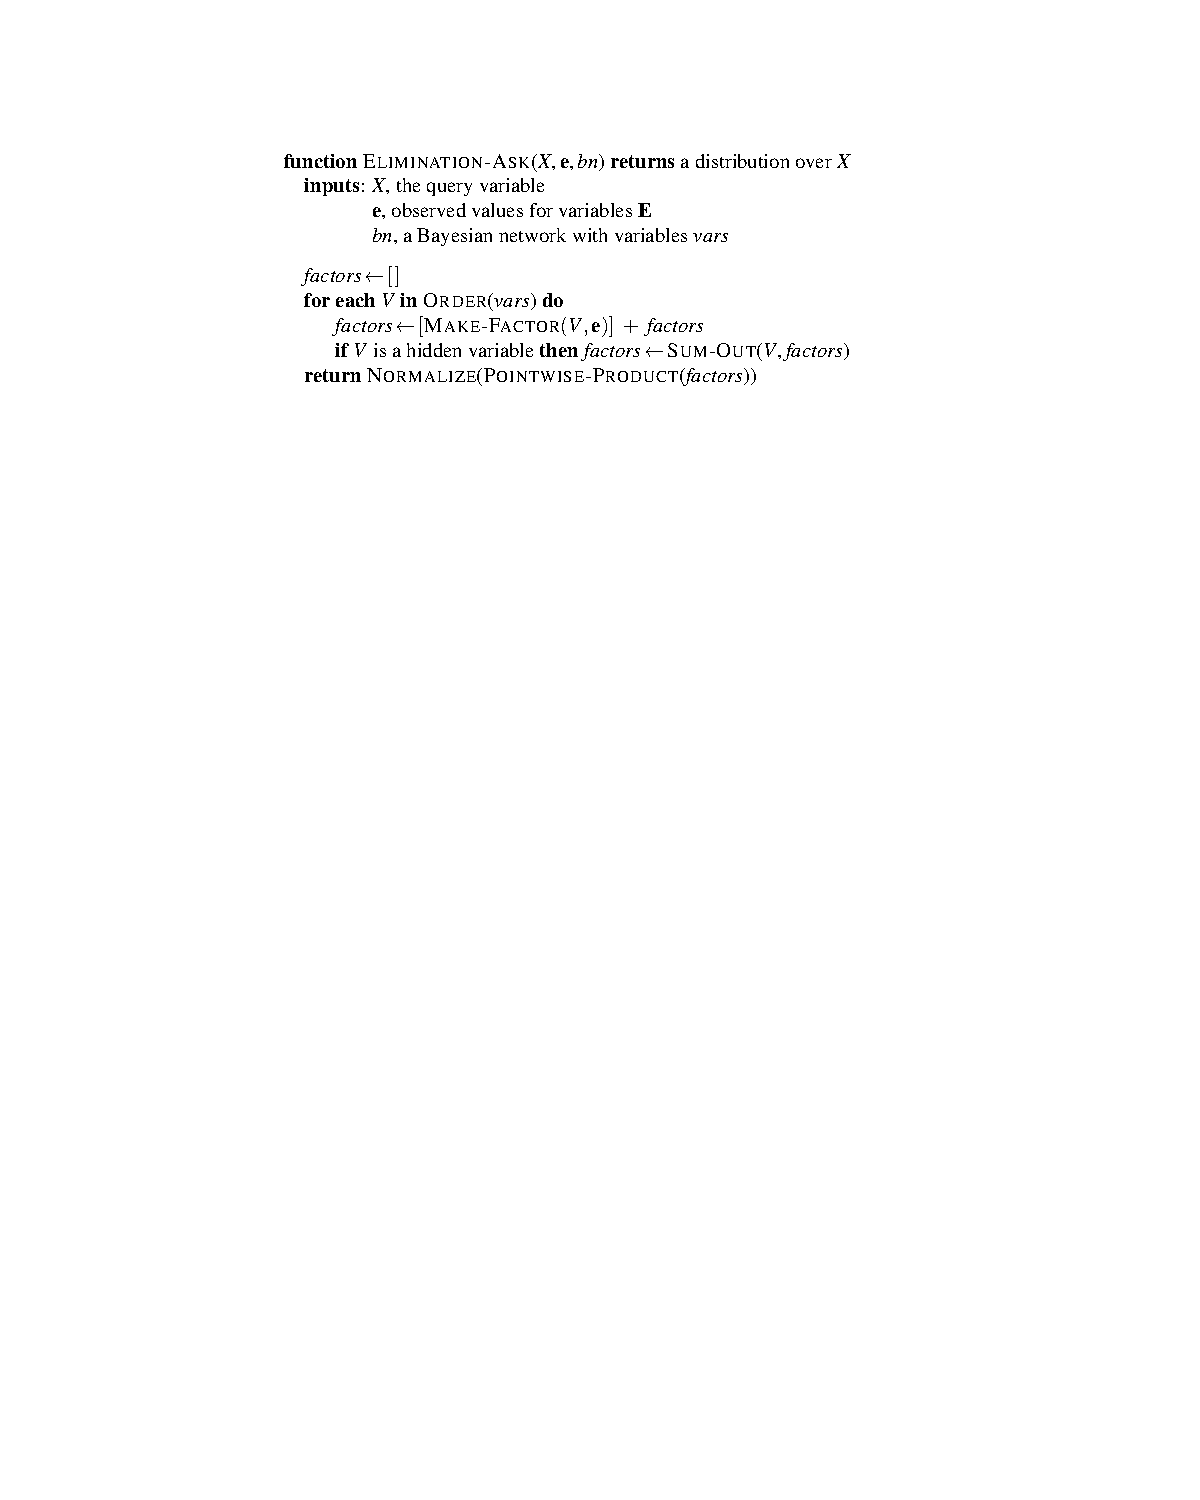
\includegraphics[alt={aima fig 13_13 bayes net variable elimination algorithm},width=0.75\linewidth]{aima-fig-13_13-bayes-net-variable-elimination-algorithm.pdf}


Notes about the \texttt{order} function:

\begin{itemize}
\item Any ordering works, some orderings lead to more efficient algorithms.
\item No tractable algorithm for determining optimal ordering.
\item One heuristic: eliminate whichever variable minimizes the size of the next factor to be contructed.
\item General rule: every variable that is not an ancestor of a query variable or evidence variable is irrelevant to the query.
\end{itemize}
\section{Complexity of Exact Inference in Polytrees}
\label{sec:org69a9f51}

Notice that the Alarm Bayes net is \textbf{singly connected}, a.k.a., a \textbf{polytree}:

\begin{itemize}
\item there is at mose one undirected path between any two nodes in the network.
\end{itemize}


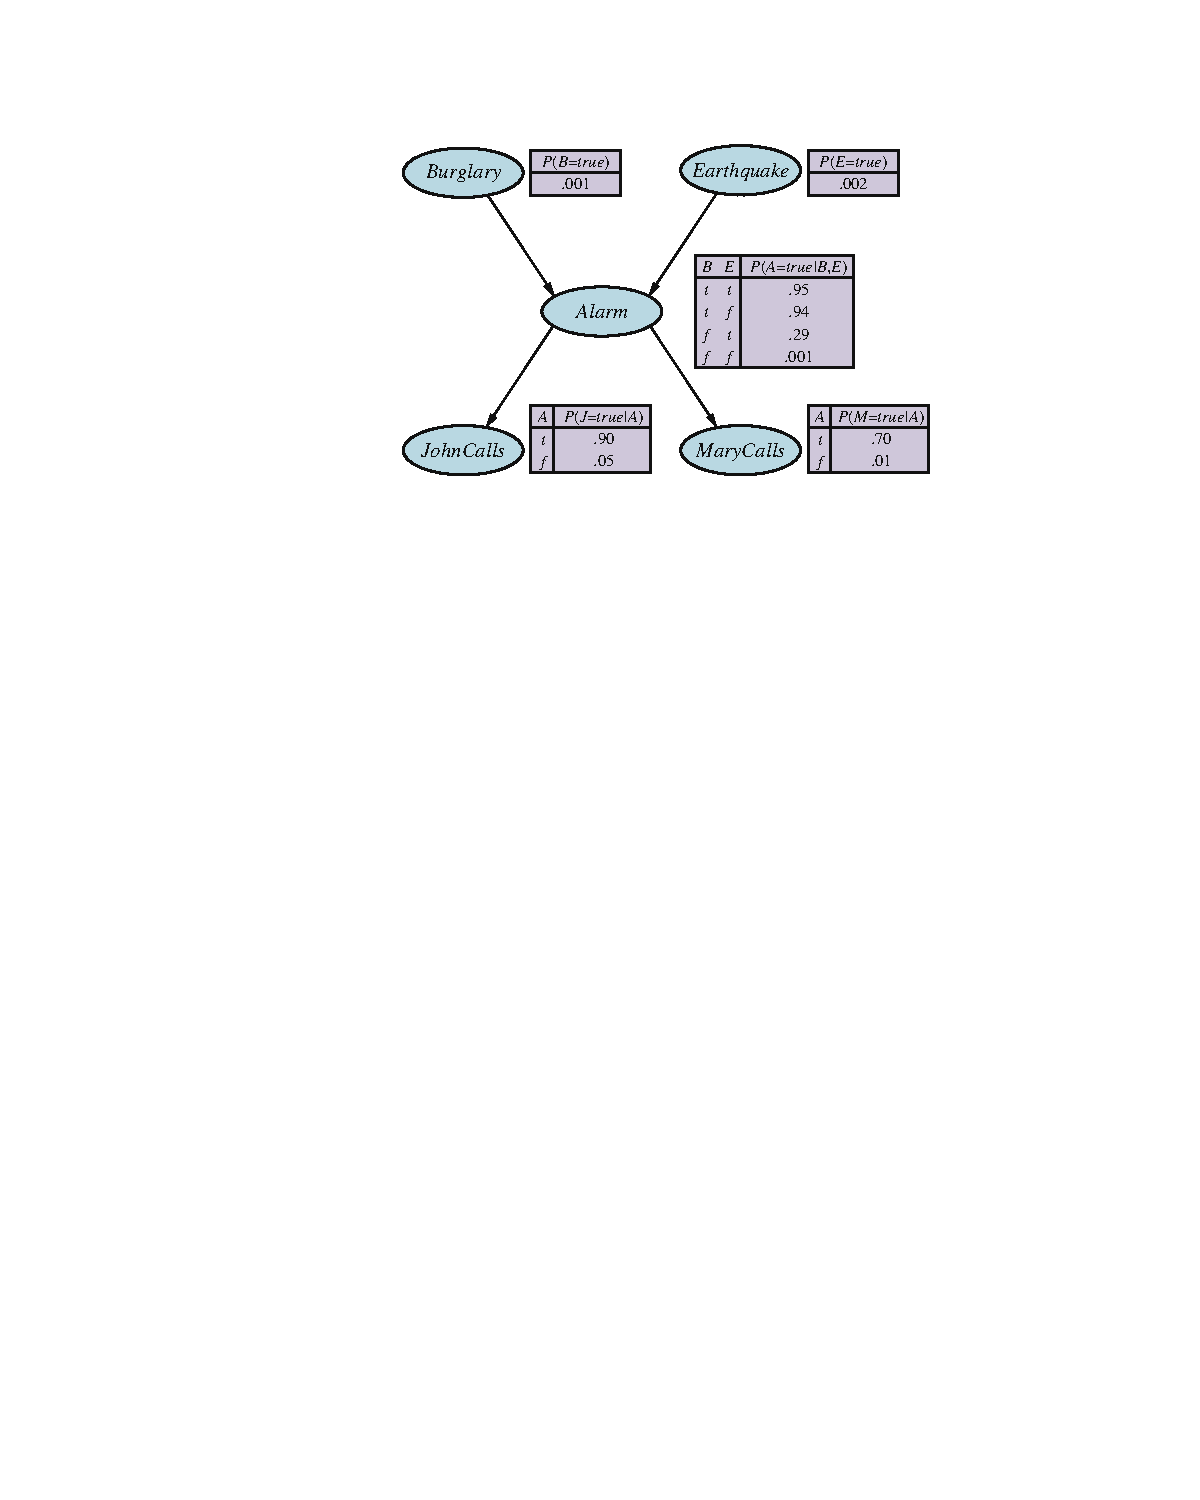
\includegraphics[alt={aima fig 13_02 bayes net alarm},height=1in]{aima-fig-13_02-bayes-net-alarm.pdf}


The time and space complexity of polytrees is linear in the size of the network.

\begin{itemize}
\item Size of network is defined as number of CPT entries.
\item If \(|parents(X_i)| \le c, \forall i \in n\) for some constant \(c\) and number of nodes \(n\), then complexity is also linear in number of nodes.
\end{itemize}
\section{Complexity of Exact Inference in Multiply-connected Networks}
\label{sec:orgfdbfb8e}

Now consider \textbf{multiply-connected} networks such as the car insurance network:


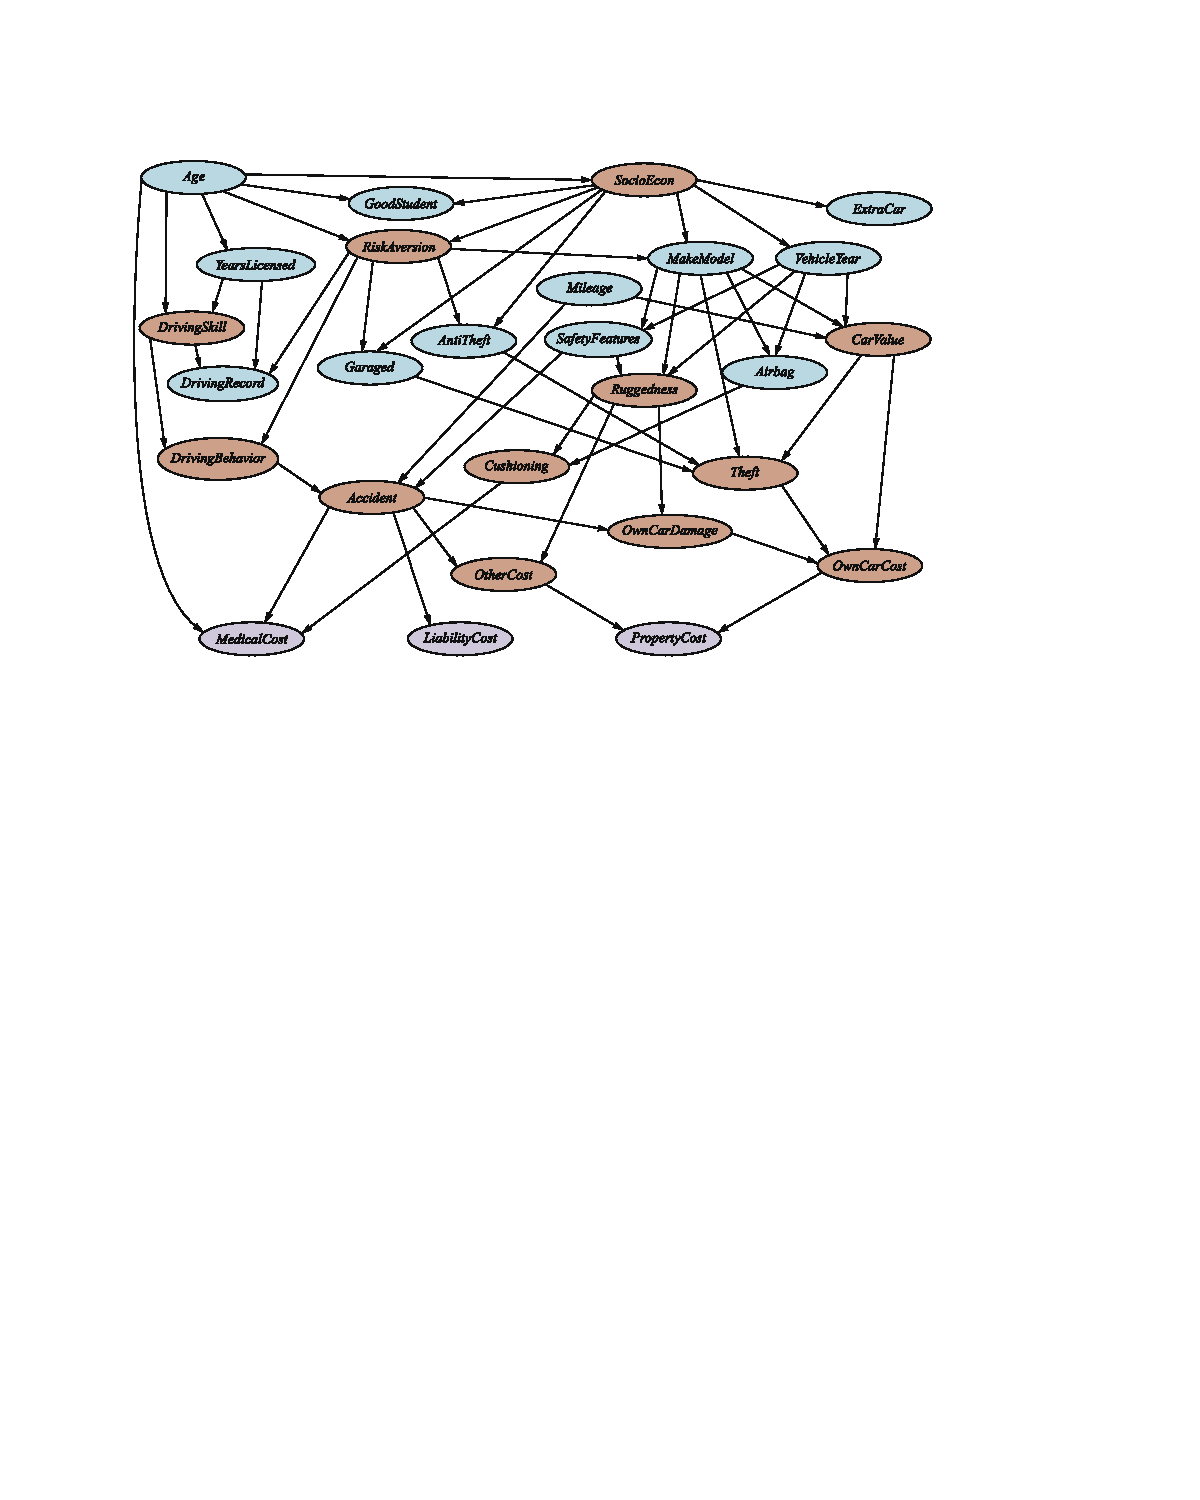
\includegraphics[alt={aima fig 13_09 bayes net car insurance},height=1in]{aima-fig-13_09-bayes-net-car-insurance.pdf}


\begin{itemize}
\item Variable elimination can have exponential worst-case time and space complexity in multiply-connected networks.
\item \textbf{Since inference in Bayes nets includes inference in propositional logic as a special case, Bayes net inference is \textbf{NP-hard}}.
\end{itemize}
\section{Closing Thoughts}
\label{sec:org536bb2f}

\begin{itemize}
\item A Bayesian network is a directed acyclic graph whose nodes correspond to random variables; each node has a conditional distribution for the node, given its parents.

\item Bayesian networks provide a concise way to represent conditional independence rela- tionships in the domain.

\item A Bayesian network specifies a joint probability distribution over its variables. The probability of any given assignment to all the variables is defined as the product of the corresponding entries in the local conditional distributions. A Bayesian network is often exponentially smaller than an explicitly enumerated joint distribution.

\item Many conditional distributions can be represented compactly by canonical families of distributions. Hybrid Bayesian networks, which include both discrete and continuous variables, use a variety of canonical distributions.
\end{itemize}
\end{document}
